\newpage
%附录
\appendix
%附录需重新起页,论文附录至少应包括参赛论文的所有源程序代码,如实际使用的软件名称、命令和编写的全部可运行的源程序(含EXCEL、SPSS等软件的交互命令);通常还应包括自主查阅使用的数据等资料。赛题中提供的数据不要放在附录。如果缺少必要的源程序或程序不能运行(或者运行结果与正文不符),可能会被取消评奖资格。如果确实没有源程序,也应在论文附录中明确说明“本论文没有源程序”。 	

\section{代码程序}
% 插入Python代码
\lstinputlisting[style=Python, caption={问题一所需Python代码}]{code/code_1.py}

\lstinputlisting[style=Python, caption={问题二所需Python代码}]{code/code_2.py}

\lstinputlisting[style=Python, caption={问题三所需Python代码}]{code/code_3.py}


\section{详细图表}

\setcounter{figure}{0}
\setcounter{table}{0}

\subsection*{问题一详细数据表}

\begin{figure}[h]%[h]:固定作用
	\centering%置中
	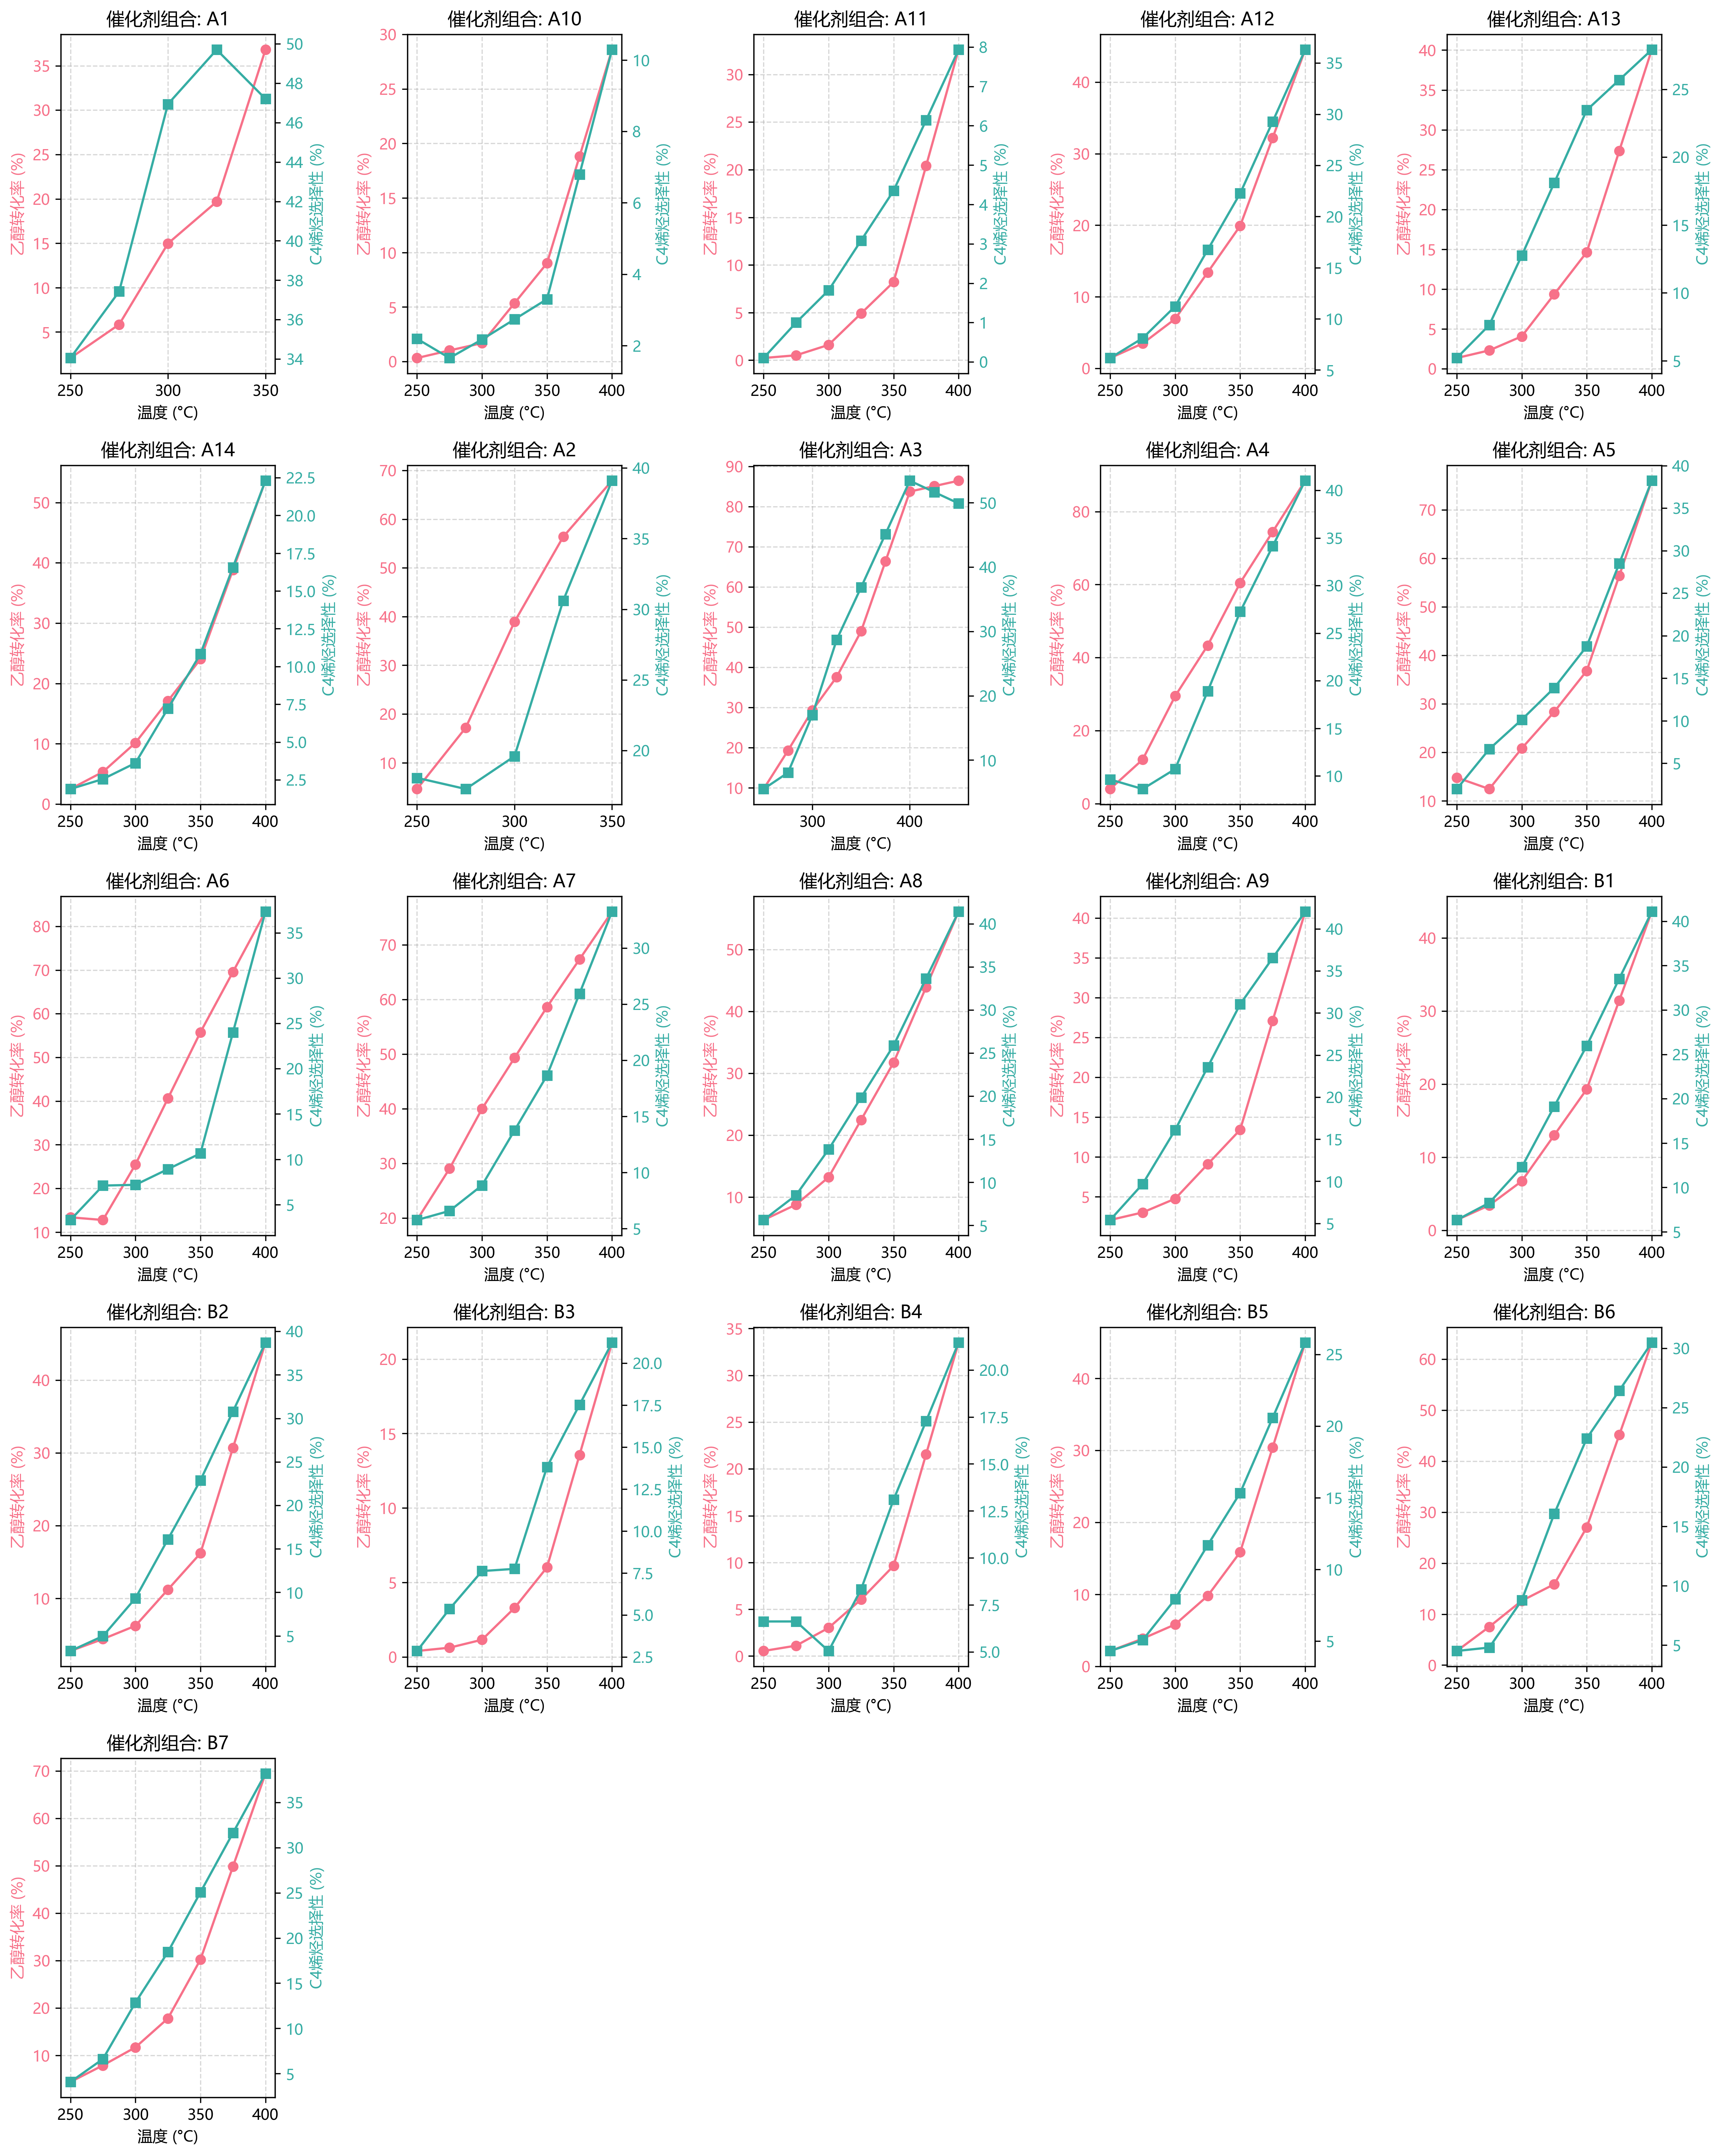
\includegraphics [scale=0.4]{图/1-1-1.png}
	\caption{乙醇转化率和C4烯烃选择性与温度的关系} 
	\label{fig:1}
\end{figure}

\begin{table}[!htbp]
	\caption{催化剂组合在不同温度下的乙醇转化率与C4烯烃选择性相关系数(部分)}
	\centering
	\begin{tabular}{c c c}
		\hline
		\multicolumn{1}{c}{催化剂组合} & \multicolumn{1}{c}{乙醇转化率-温度 (r)} & \multicolumn{1}{c}{C4烯烃选择性-温度 (r)} \\
		\hline
		A1  & 0.9655 & 0.8871 \\
		A2  & 0.9950 & 0.9143 \\
		B1  & 0.9621 & 0.9858 \\
		B2  & 0.9293 & 0.9848 \\
		\hline
	\end{tabular}
	\label{tab:1}
\end{table}

\begin{figure}[h]%[h]:固定作用
	\centering%置中
	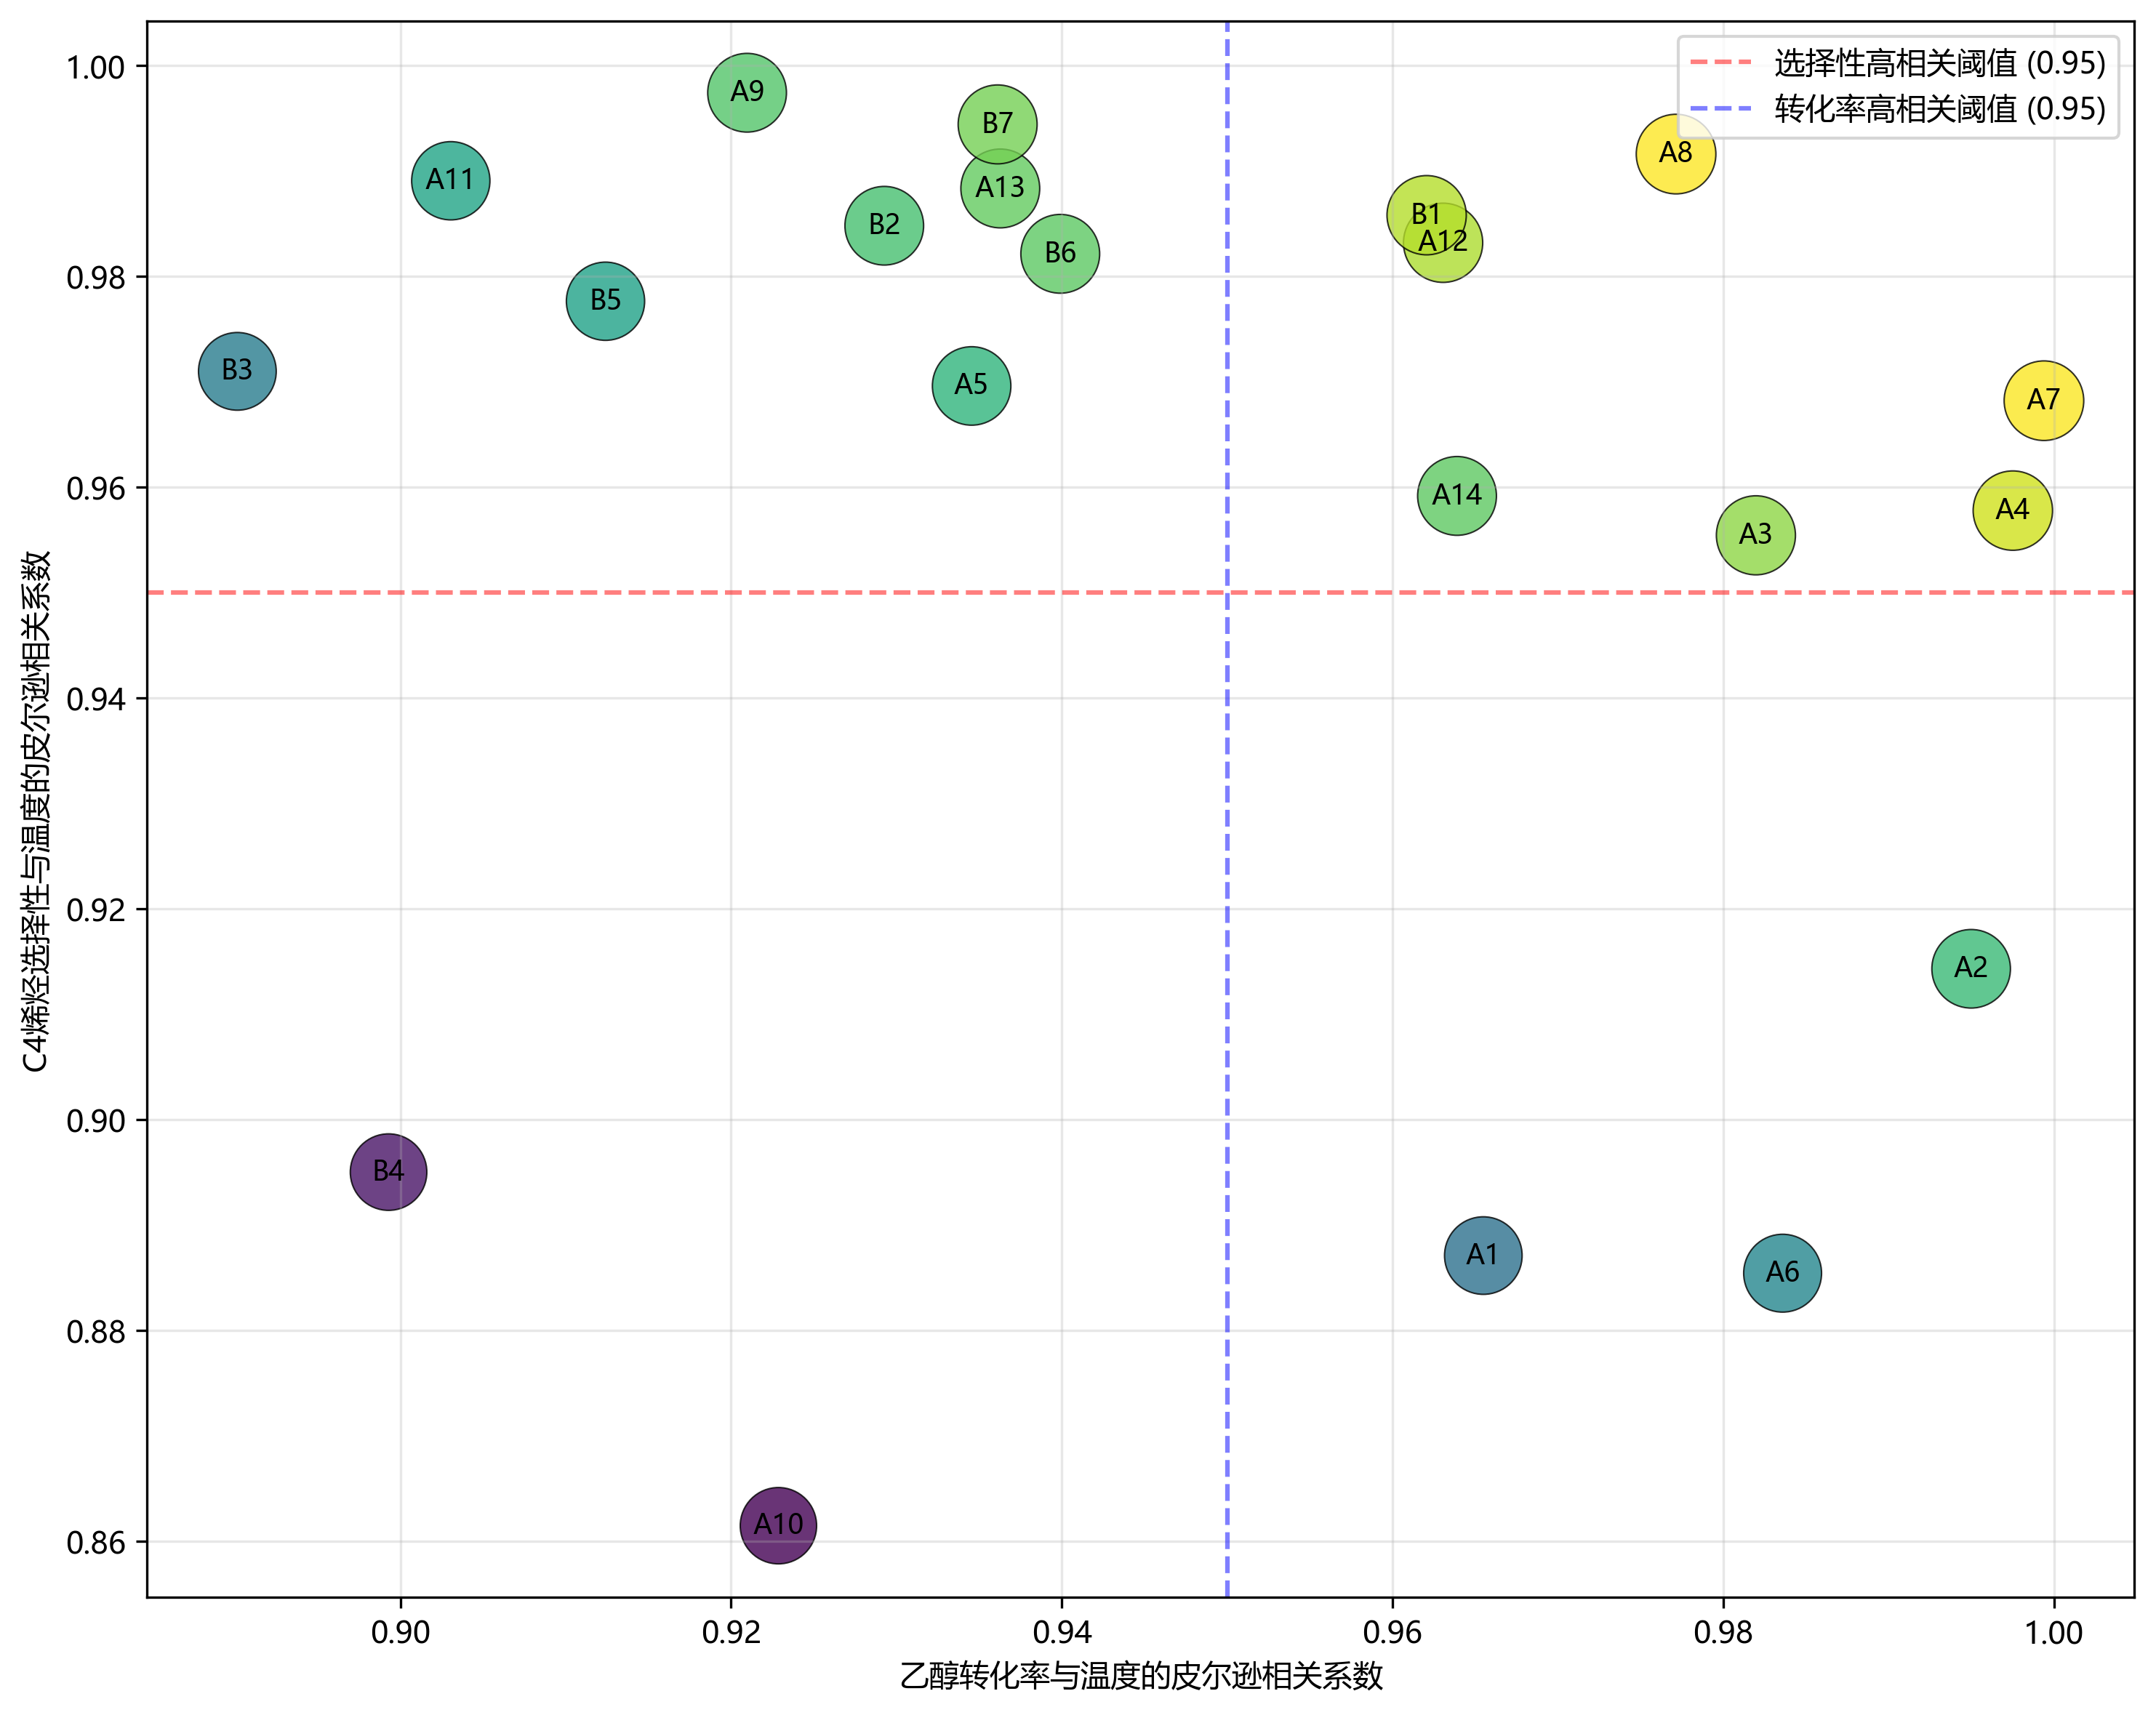
\includegraphics [scale=0.6]{图/1-2-2.png}
	\caption{各催化剂组合双指标相关性分布} 
	\label{fig:1}
\end{figure}

\begin{figure}[h]%[h]:固定作用
	\centering%置中
	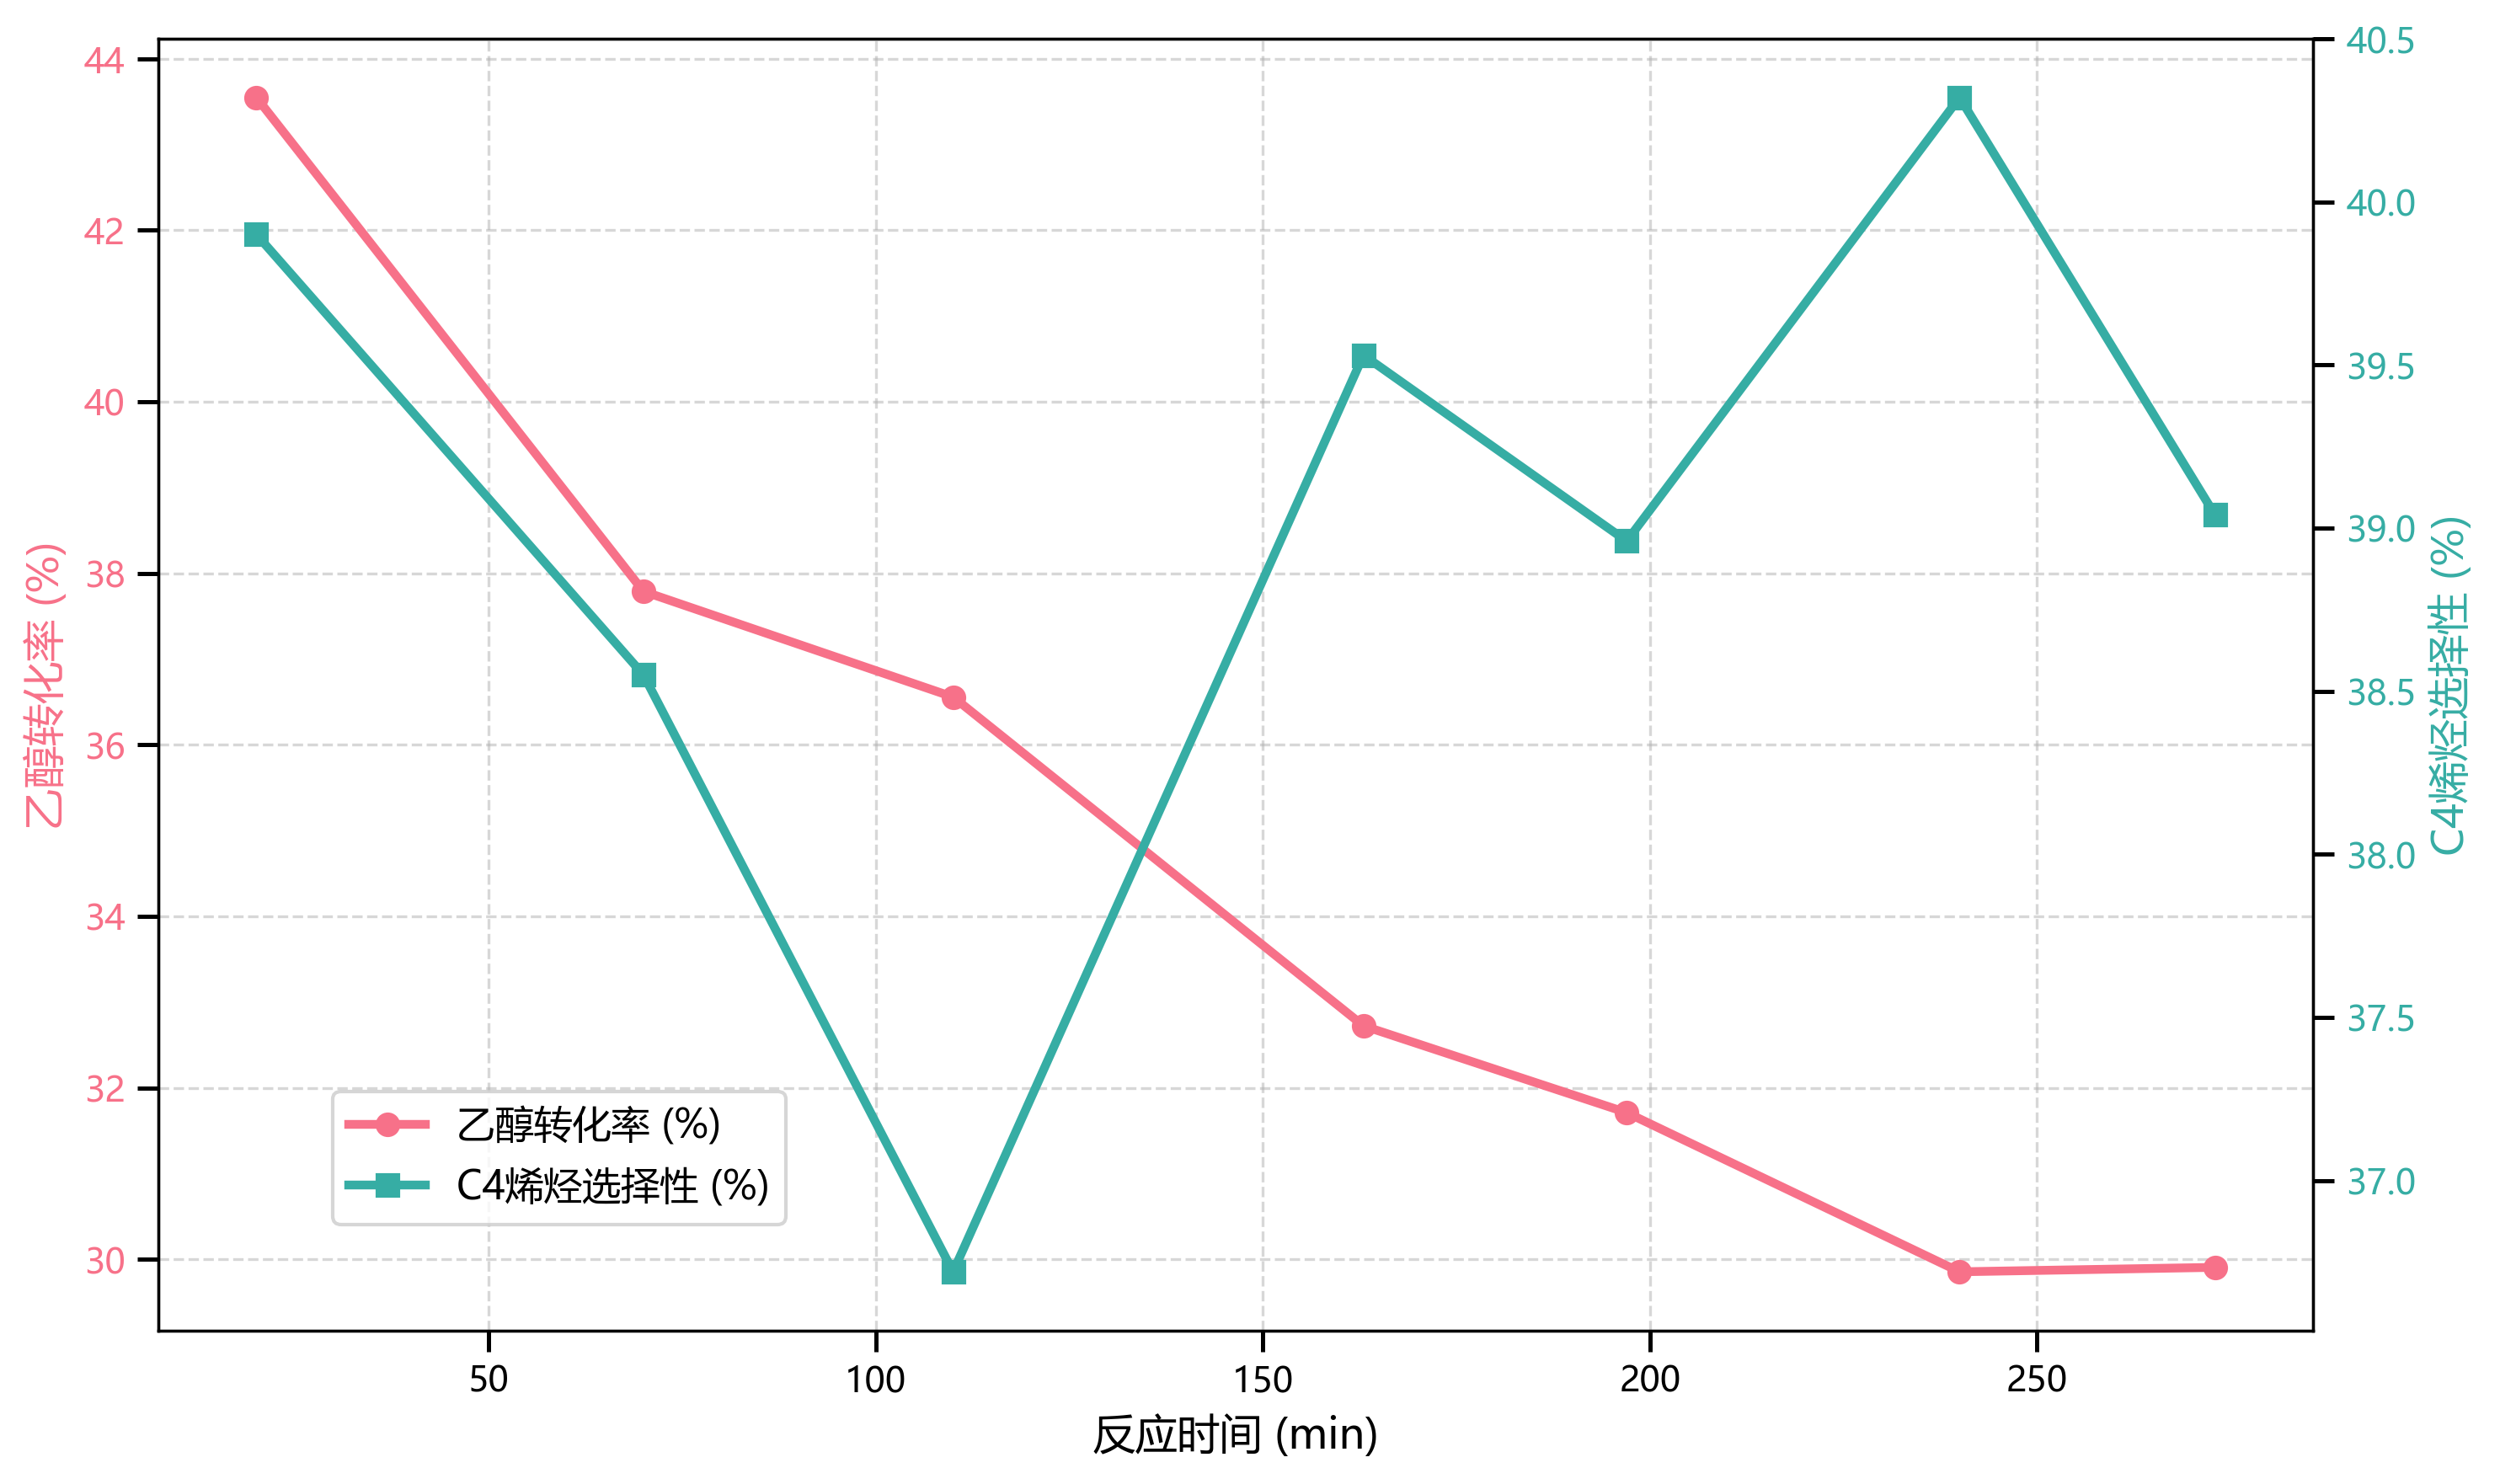
\includegraphics [scale=0.6]{图/1-2-1.png}
	\caption{350°C 下催化剂组合稳定性测试(不同反应时间性能变化)} 
	\label{fig:1}
\end{figure}

\newpage

\subsection*{问题二详细数据表}

\begin{figure}[h]%[h]:固定作用
	\centering%置中
	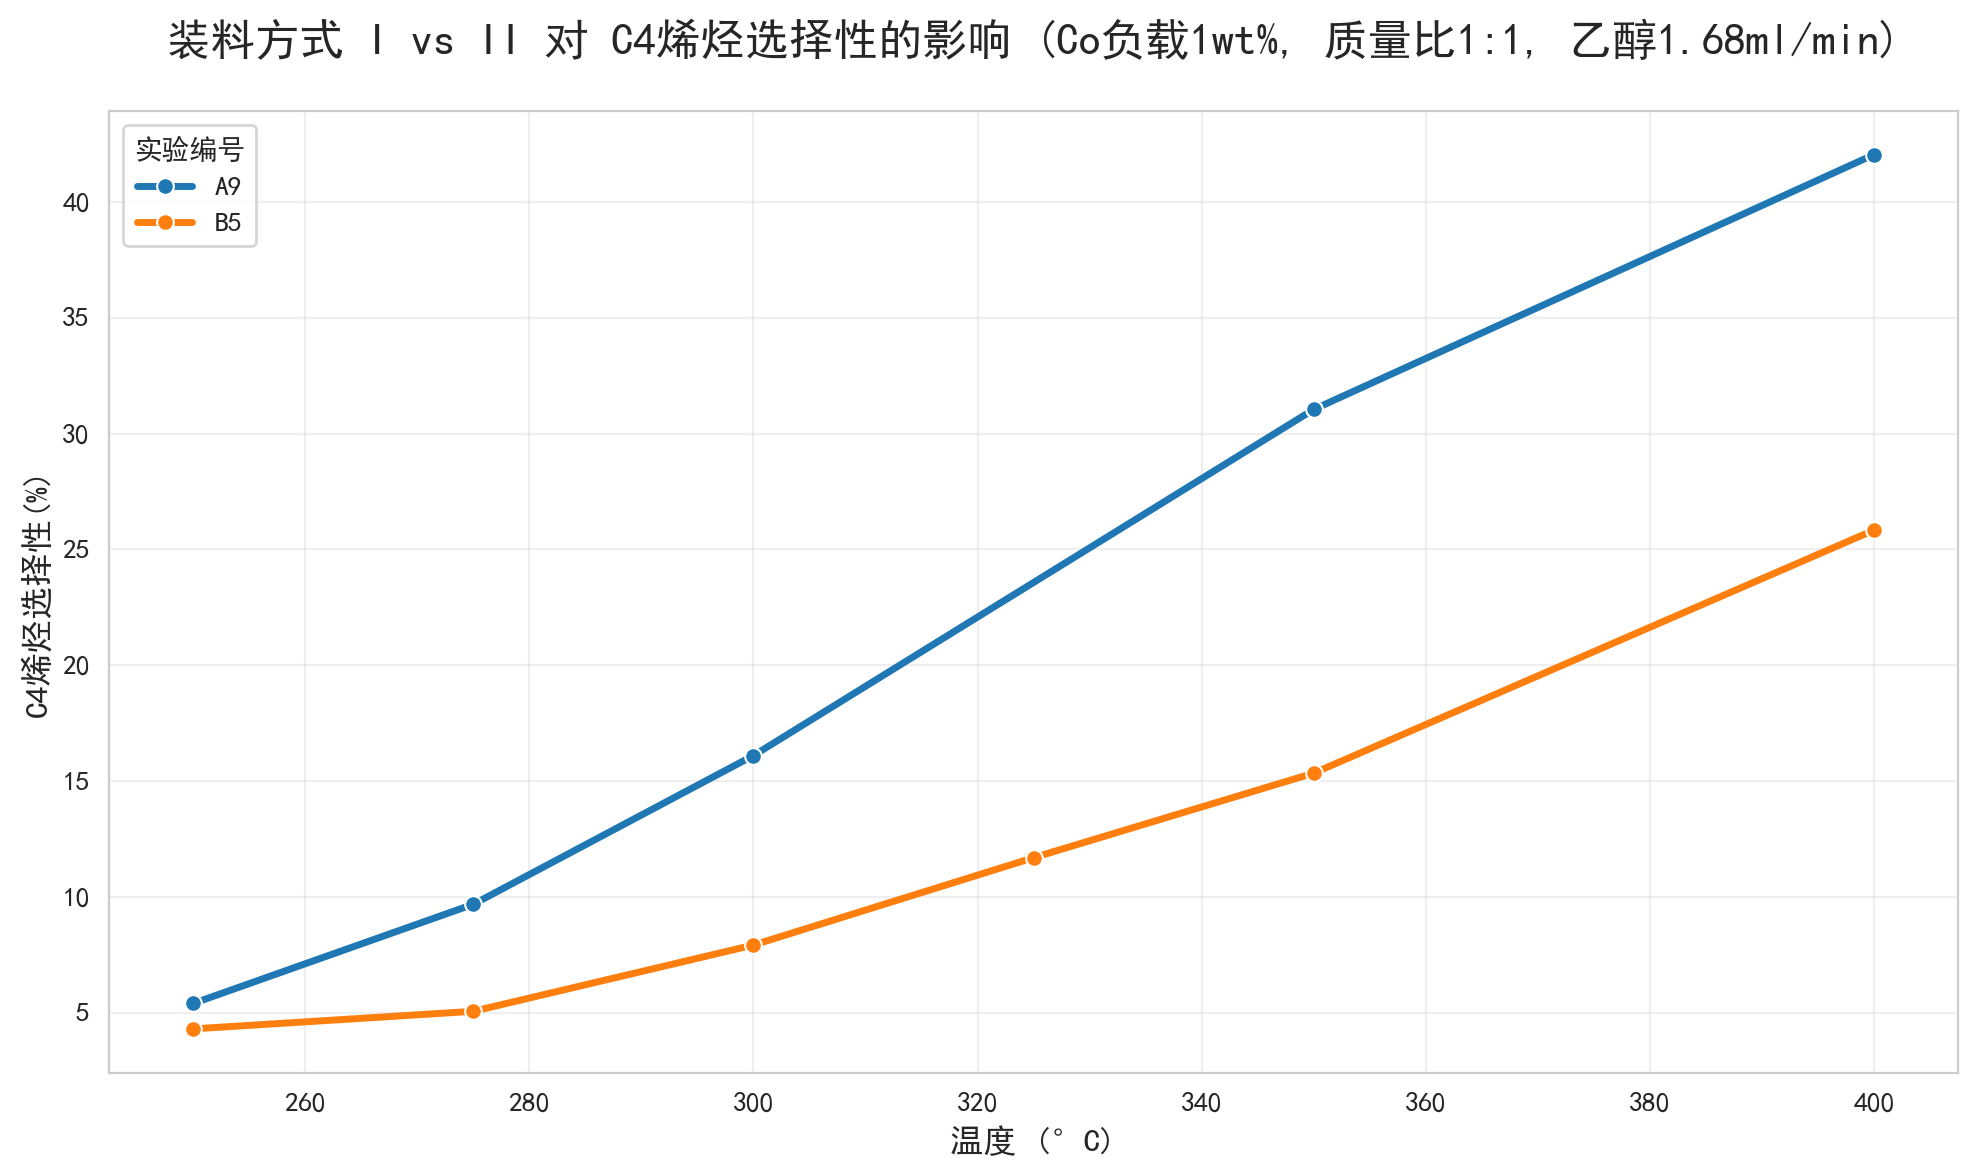
\includegraphics [scale=0.6]{图/2-1-2-1.png}
	\caption{装料方式对C4烯烃选择性的影响(Co负载1wt\%,质量比1:1,乙醇1.68ml/min)} 
	\label{fig:1}
\end{figure}

\newpage

\begin{figure}[h]%[h]:固定作用
	\centering%置中
	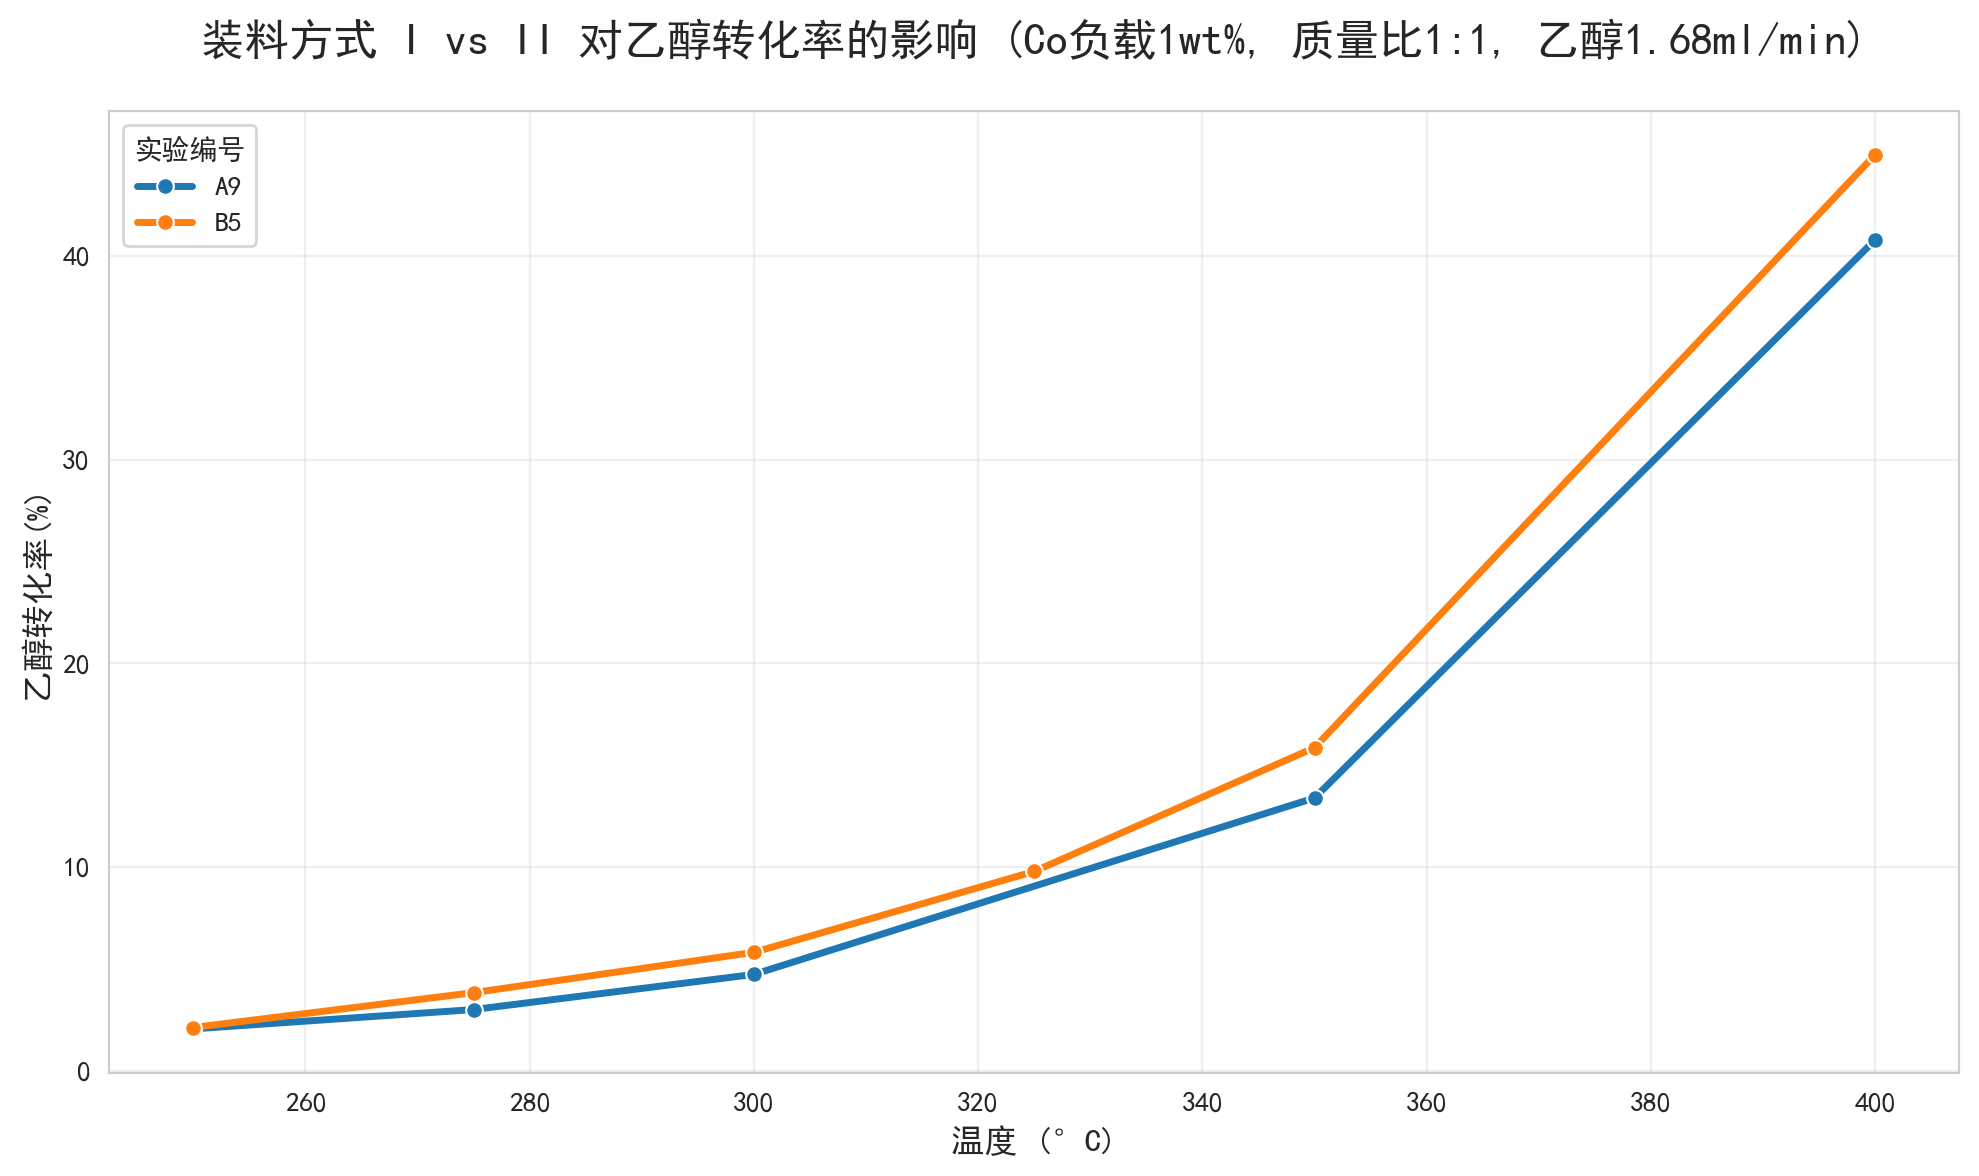
\includegraphics [scale=0.6]{图/2-1-2-2.png}
	\caption{装料方式对乙醇转化率的影响(Co负载1wt\%, 质量比1:1,乙醇1.68ml/min)} 
	\label{fig:1}
\end{figure}

\begin{figure}[h]%[h]:固定作用
	\centering%置中
	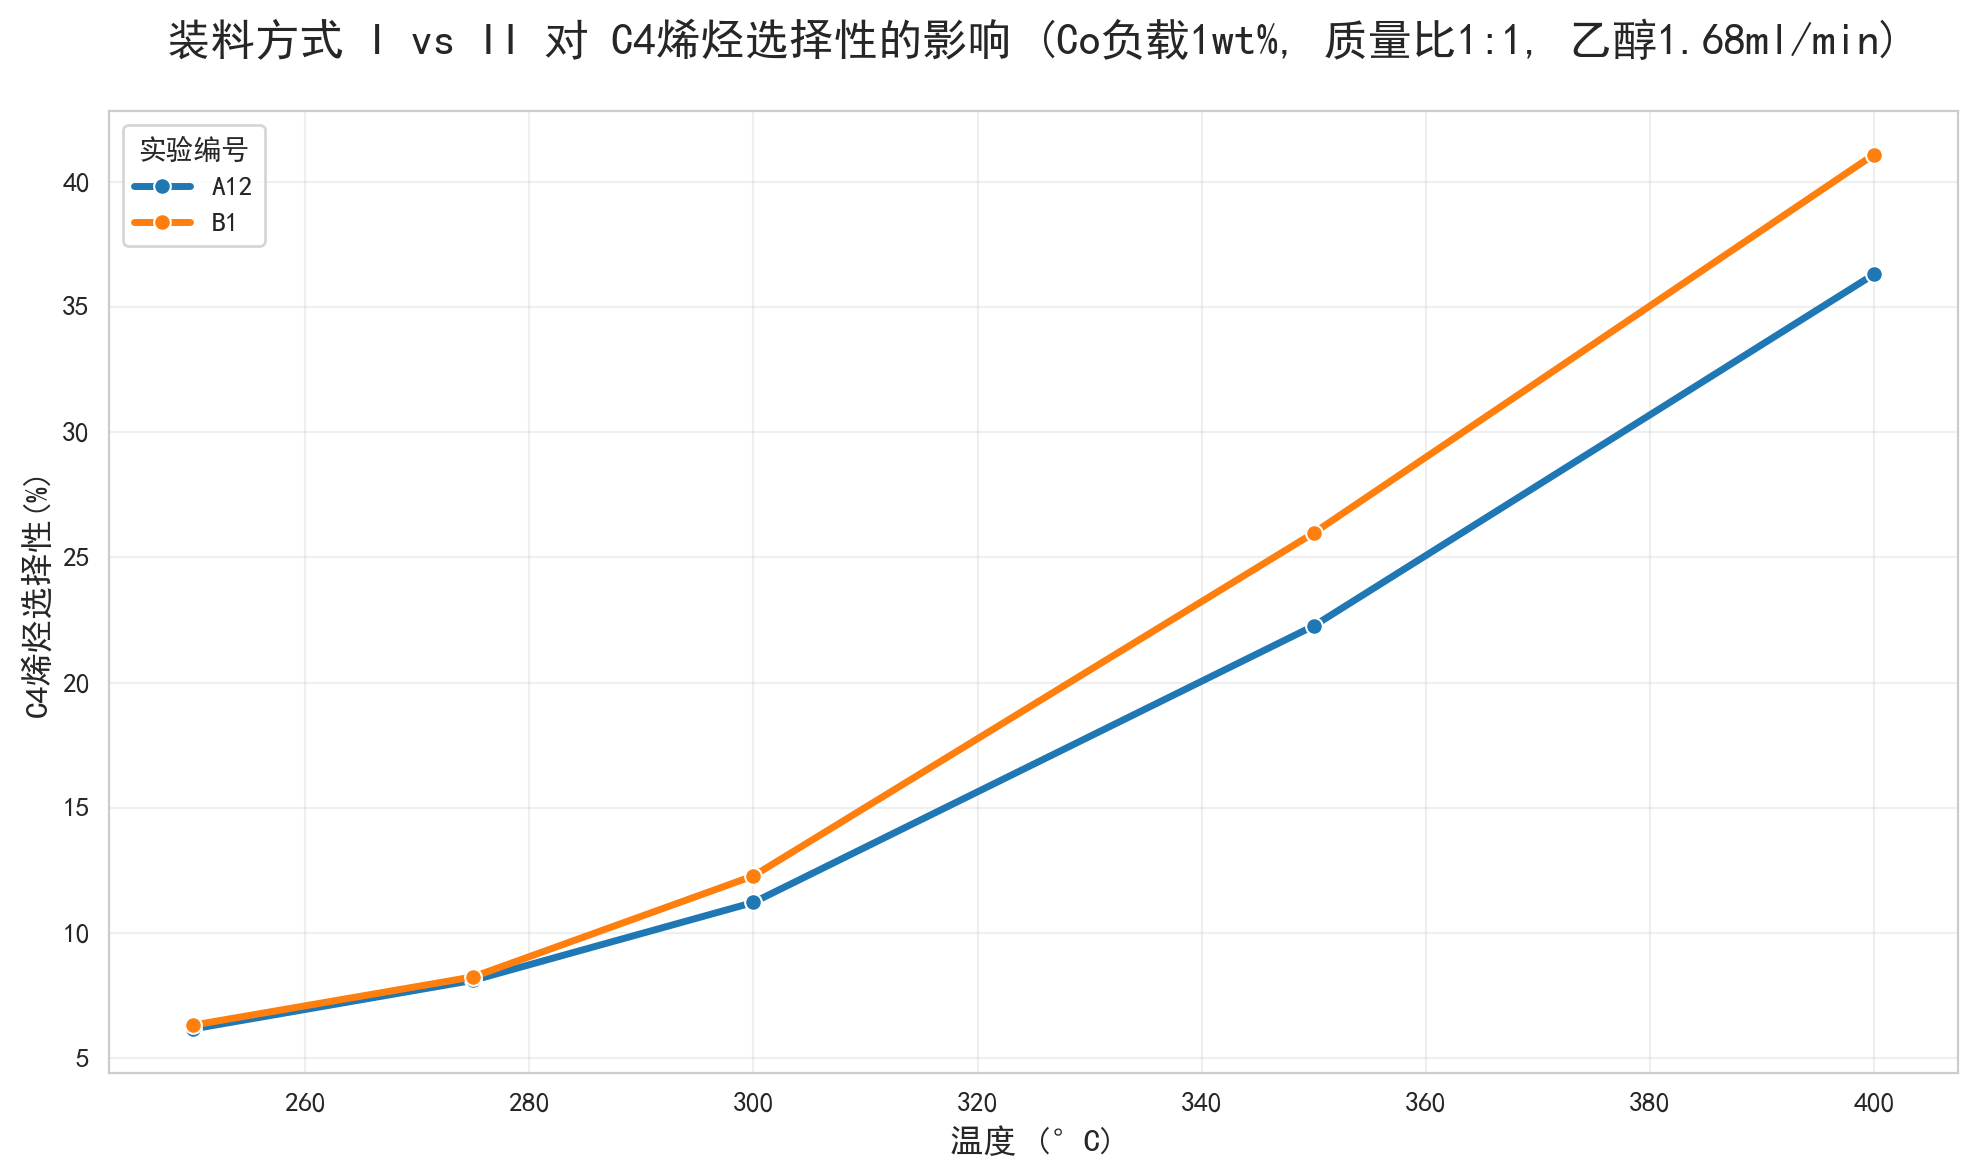
\includegraphics [scale=0.6]{图/2-1-1-1.png}
	\caption{装料方式 I vs II 对 C4烯烃选择性的影响 (Co负载1wt\%, 质量比1:1, 乙醇1.68ml/min)} 
	\label{fig:1}
\end{figure}

\begin{figure}[h]%[h]:固定作用
	\centering%置中
	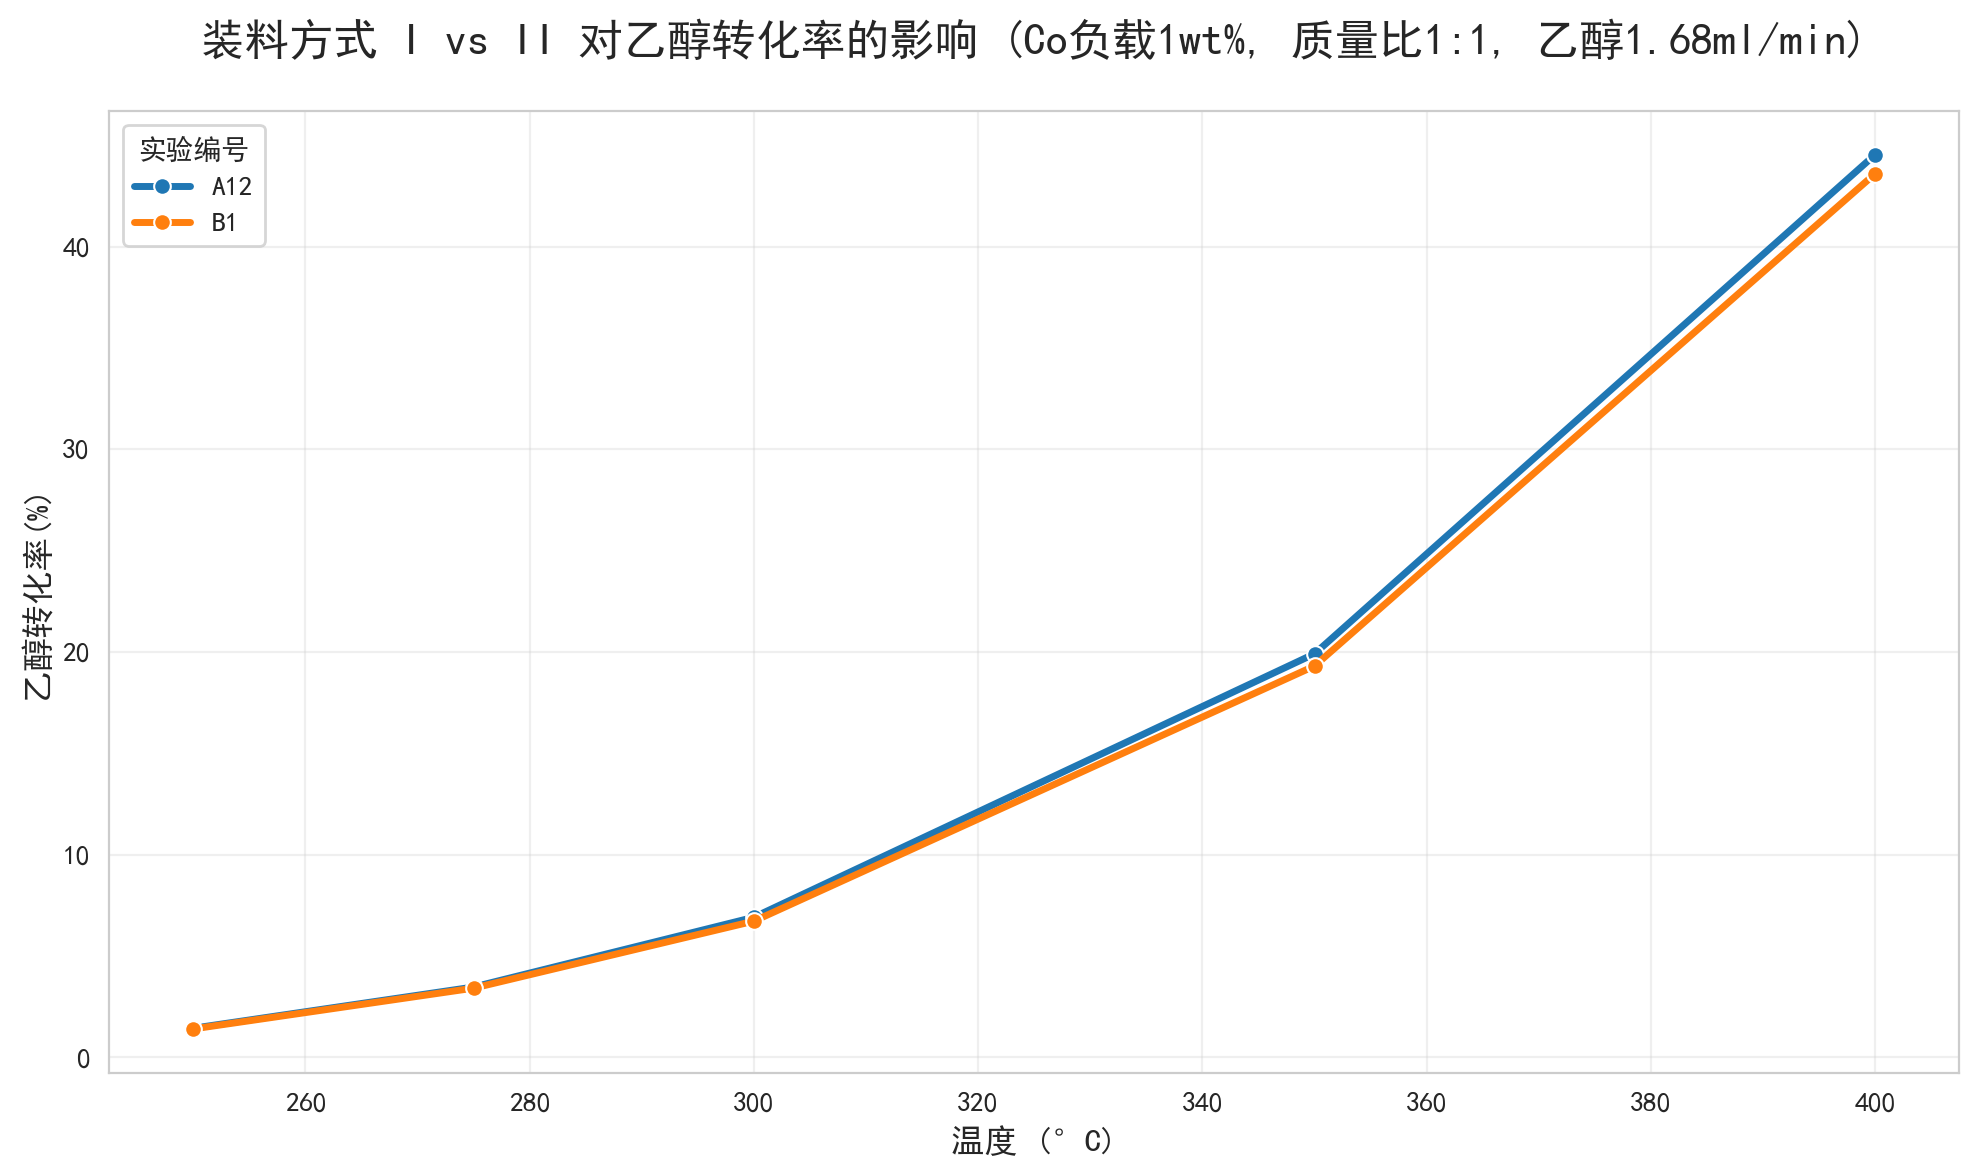
\includegraphics [scale=0.6]{图/2-1-1-2.png}
	\caption{装料方式 I vs II 对乙醇转化率的影响 (Co负载1wt\%, 质量比1:1, 乙醇1.68ml/min)} 
	\label{fig:1}
\end{figure}

\begin{figure}[h]%[h]:固定作用
	\centering%置中
	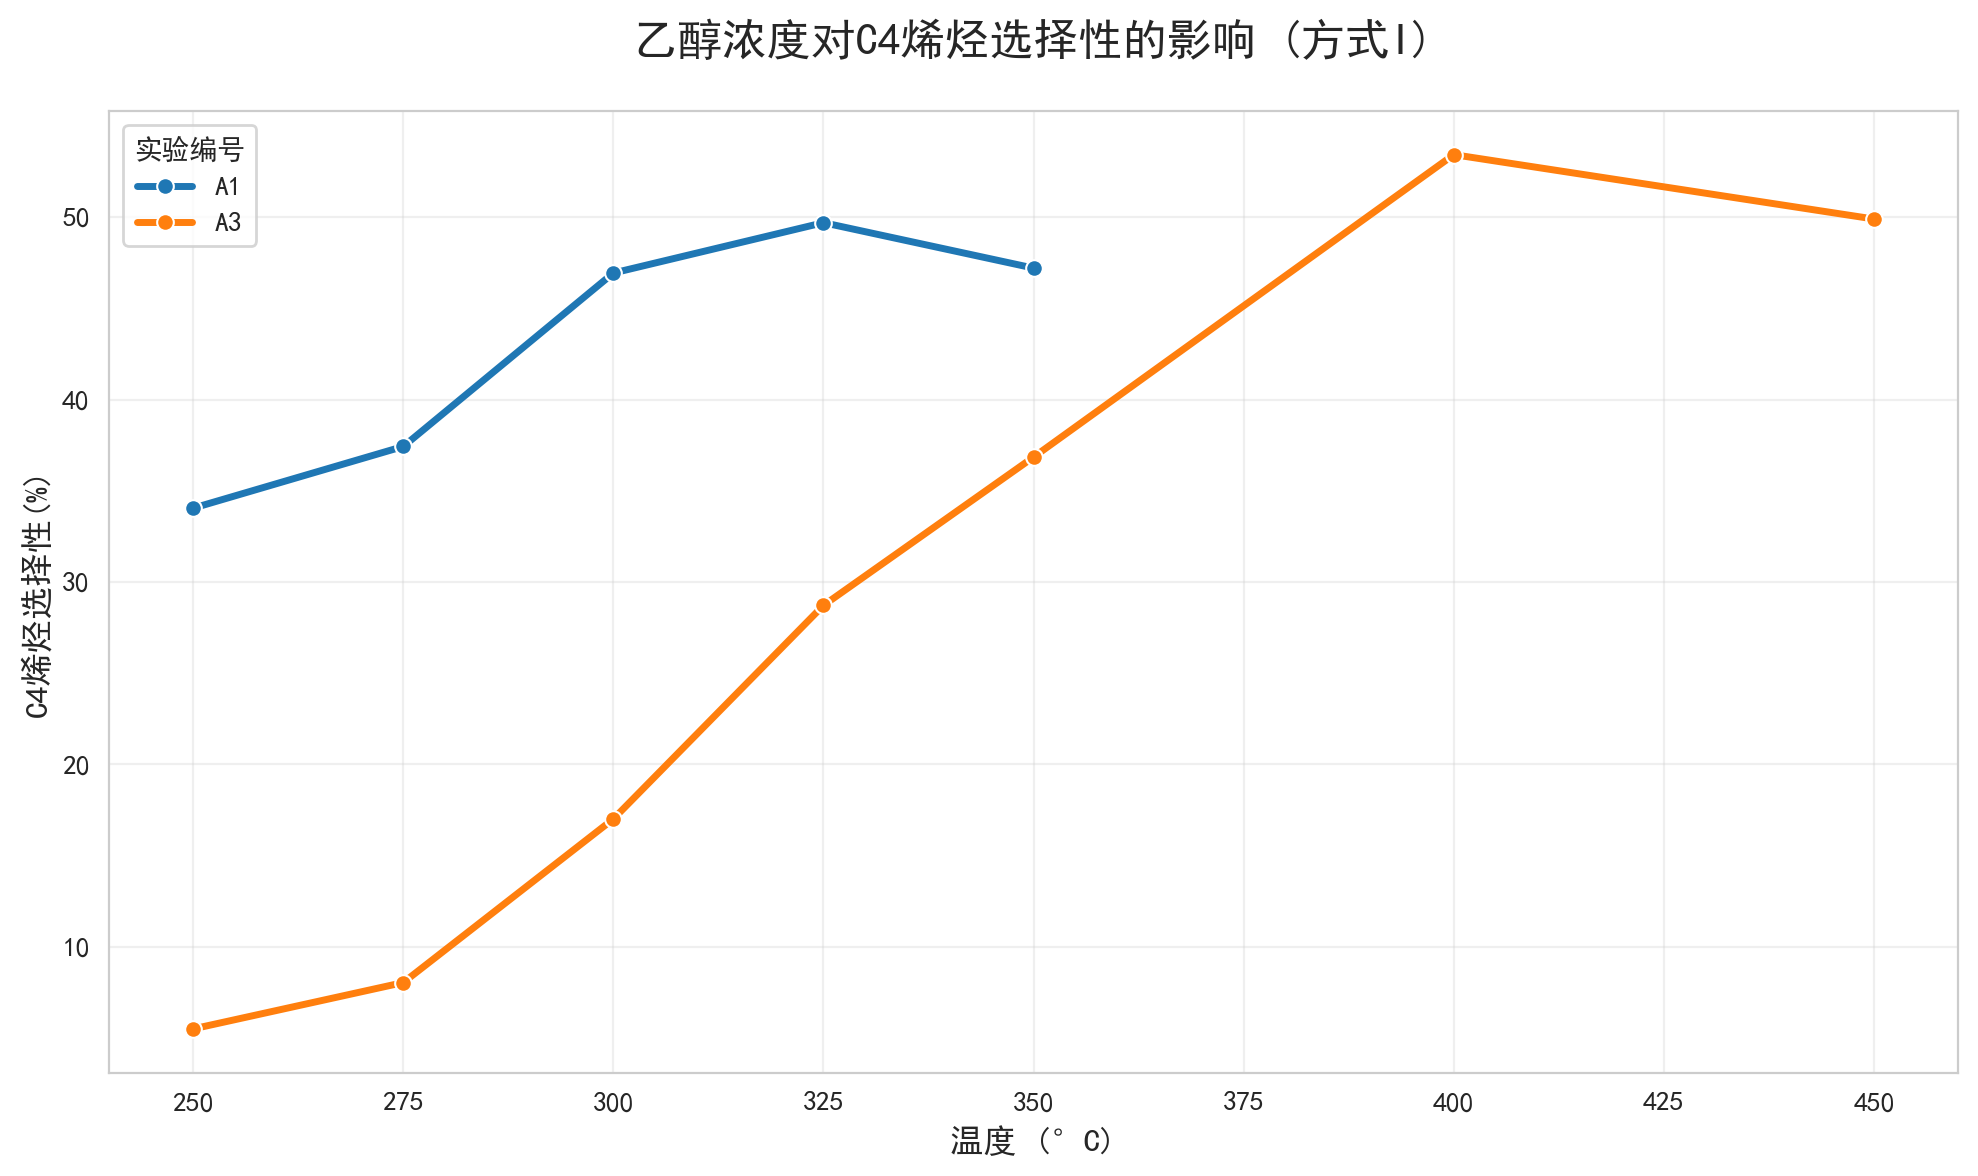
\includegraphics [scale=0.6]{图/2-2-1-1.png}
	\caption{乙醇浓度对C4烯烃选择性的影响 (方式I)} 
	\label{fig:1}
\end{figure}

\begin{figure}[h]%[h]:固定作用
	\centering%置中
	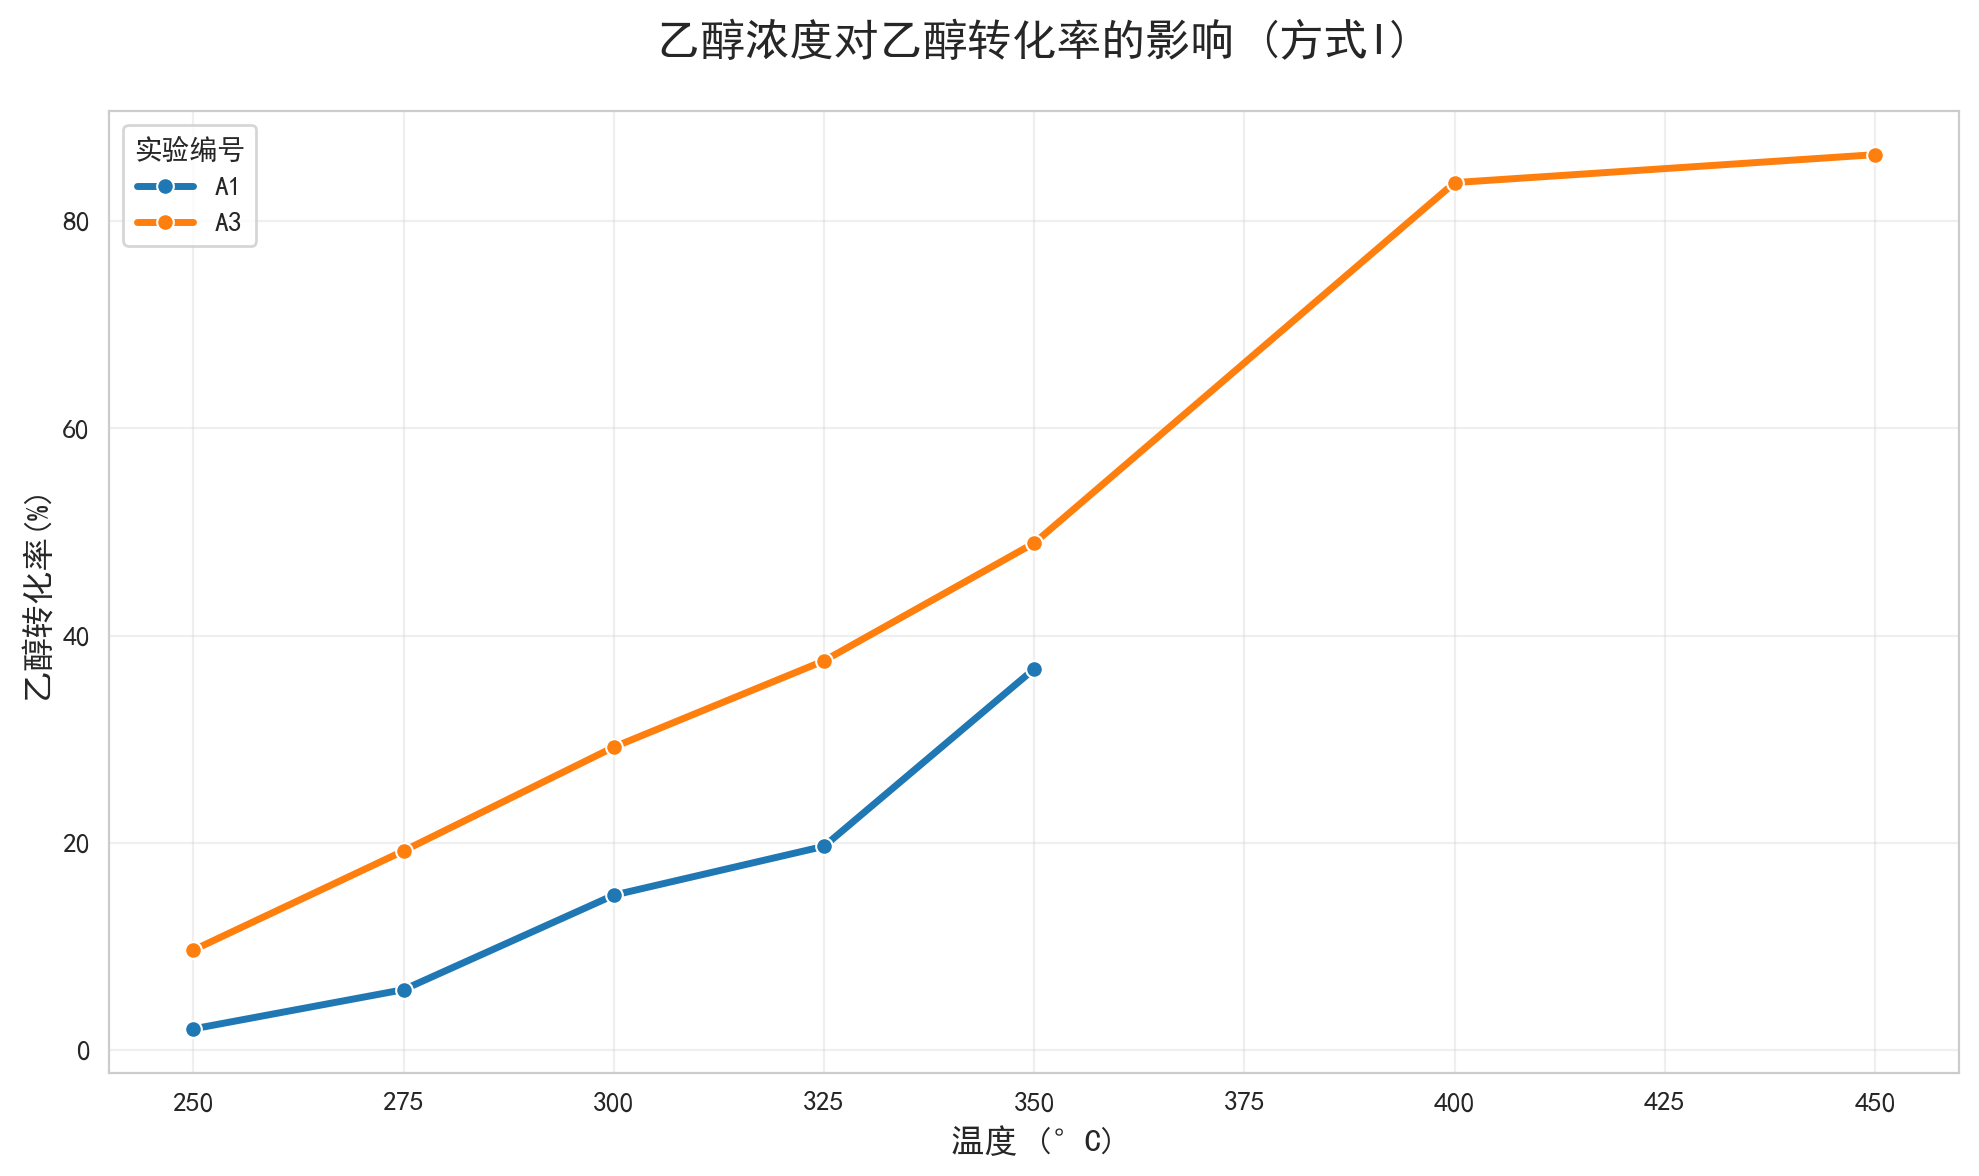
\includegraphics [scale=0.6]{图/2-2-1-2.png}
	\caption{乙醇浓度对乙醇转化率的影响 (方式I)} 
	\label{fig:1}
\end{figure}

\begin{figure}[h]%[h]:固定作用
	\centering%置中
	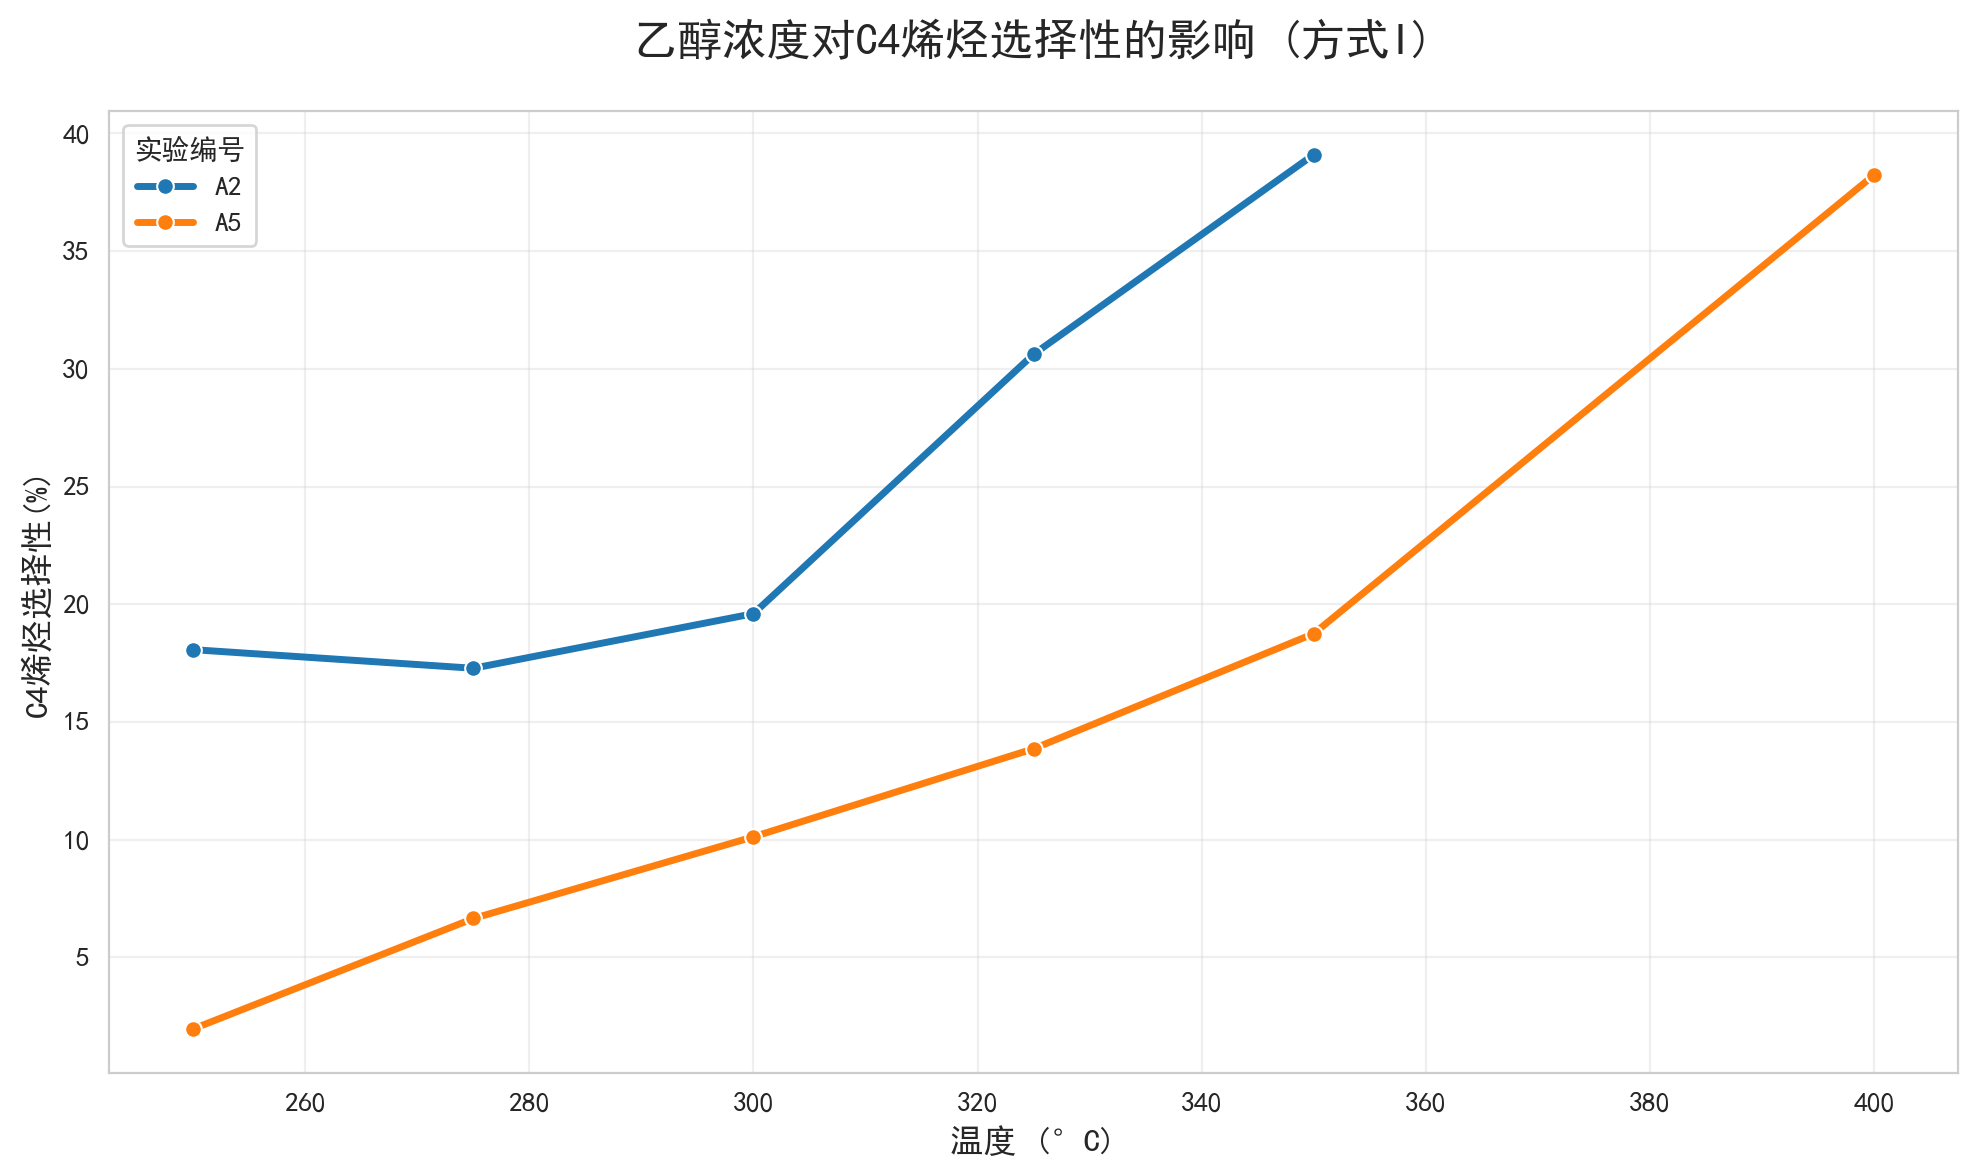
\includegraphics [scale=0.6]{图/2-2-2-1.png}
	\caption{乙醇浓度对C4烯烃选择性的影响 (方式I)} 
	\label{fig:1}
\end{figure}

\begin{figure}[h]%[h]:固定作用
	\centering%置中
	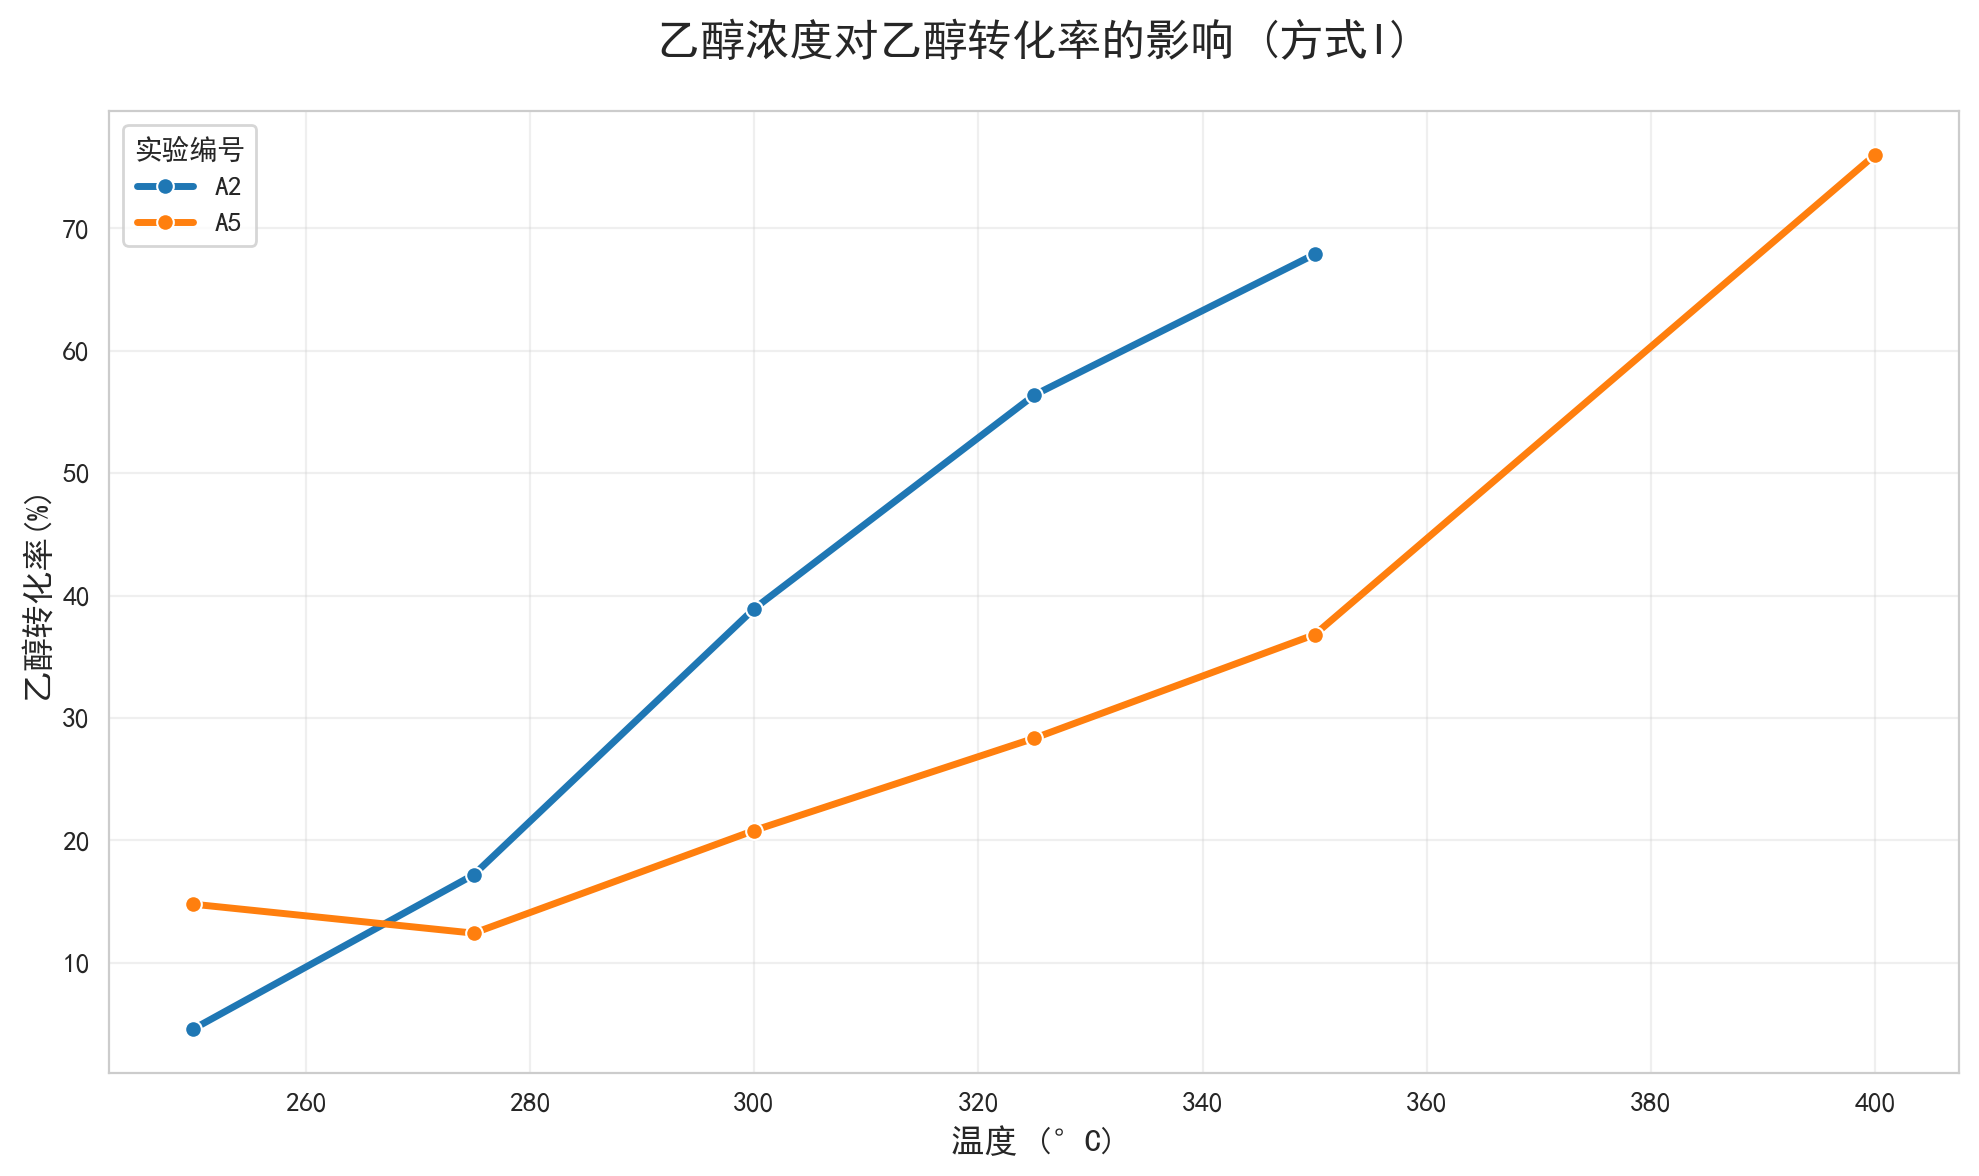
\includegraphics [scale=0.6]{图/2-2-2-2.png}
	\caption{乙醇浓度对乙醇转化率的影响 (方式I)} 
	\label{fig:1}
\end{figure}

\begin{figure}[h]%[h]:固定作用
	\centering%置中
	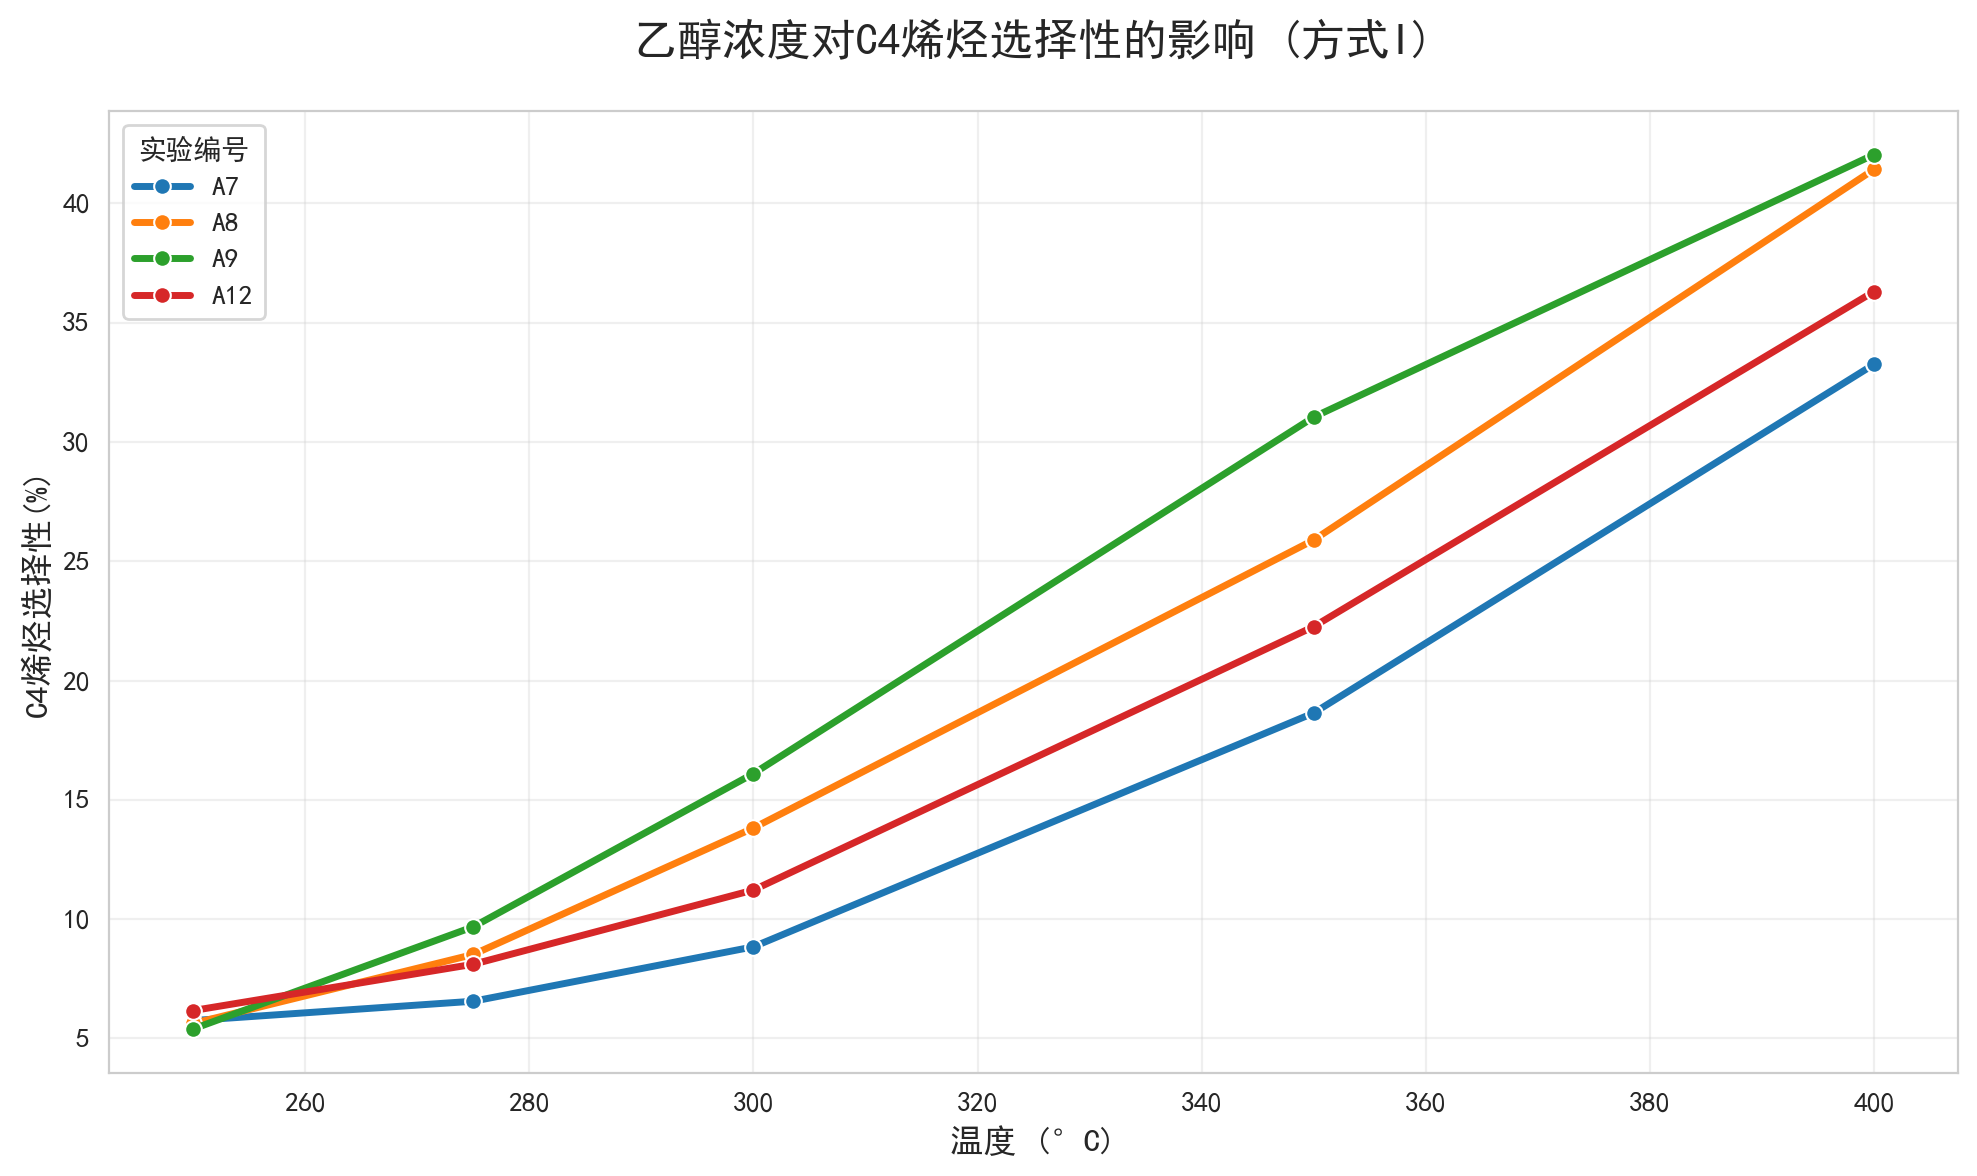
\includegraphics [scale=0.6]{图/2-2-3-1.png}
	\caption{乙醇浓度对C4烯烃选择性的影响 (方式I)} 
	\label{fig:1}
\end{figure}

\begin{figure}[h]%[h]:固定作用
	\centering%置中
	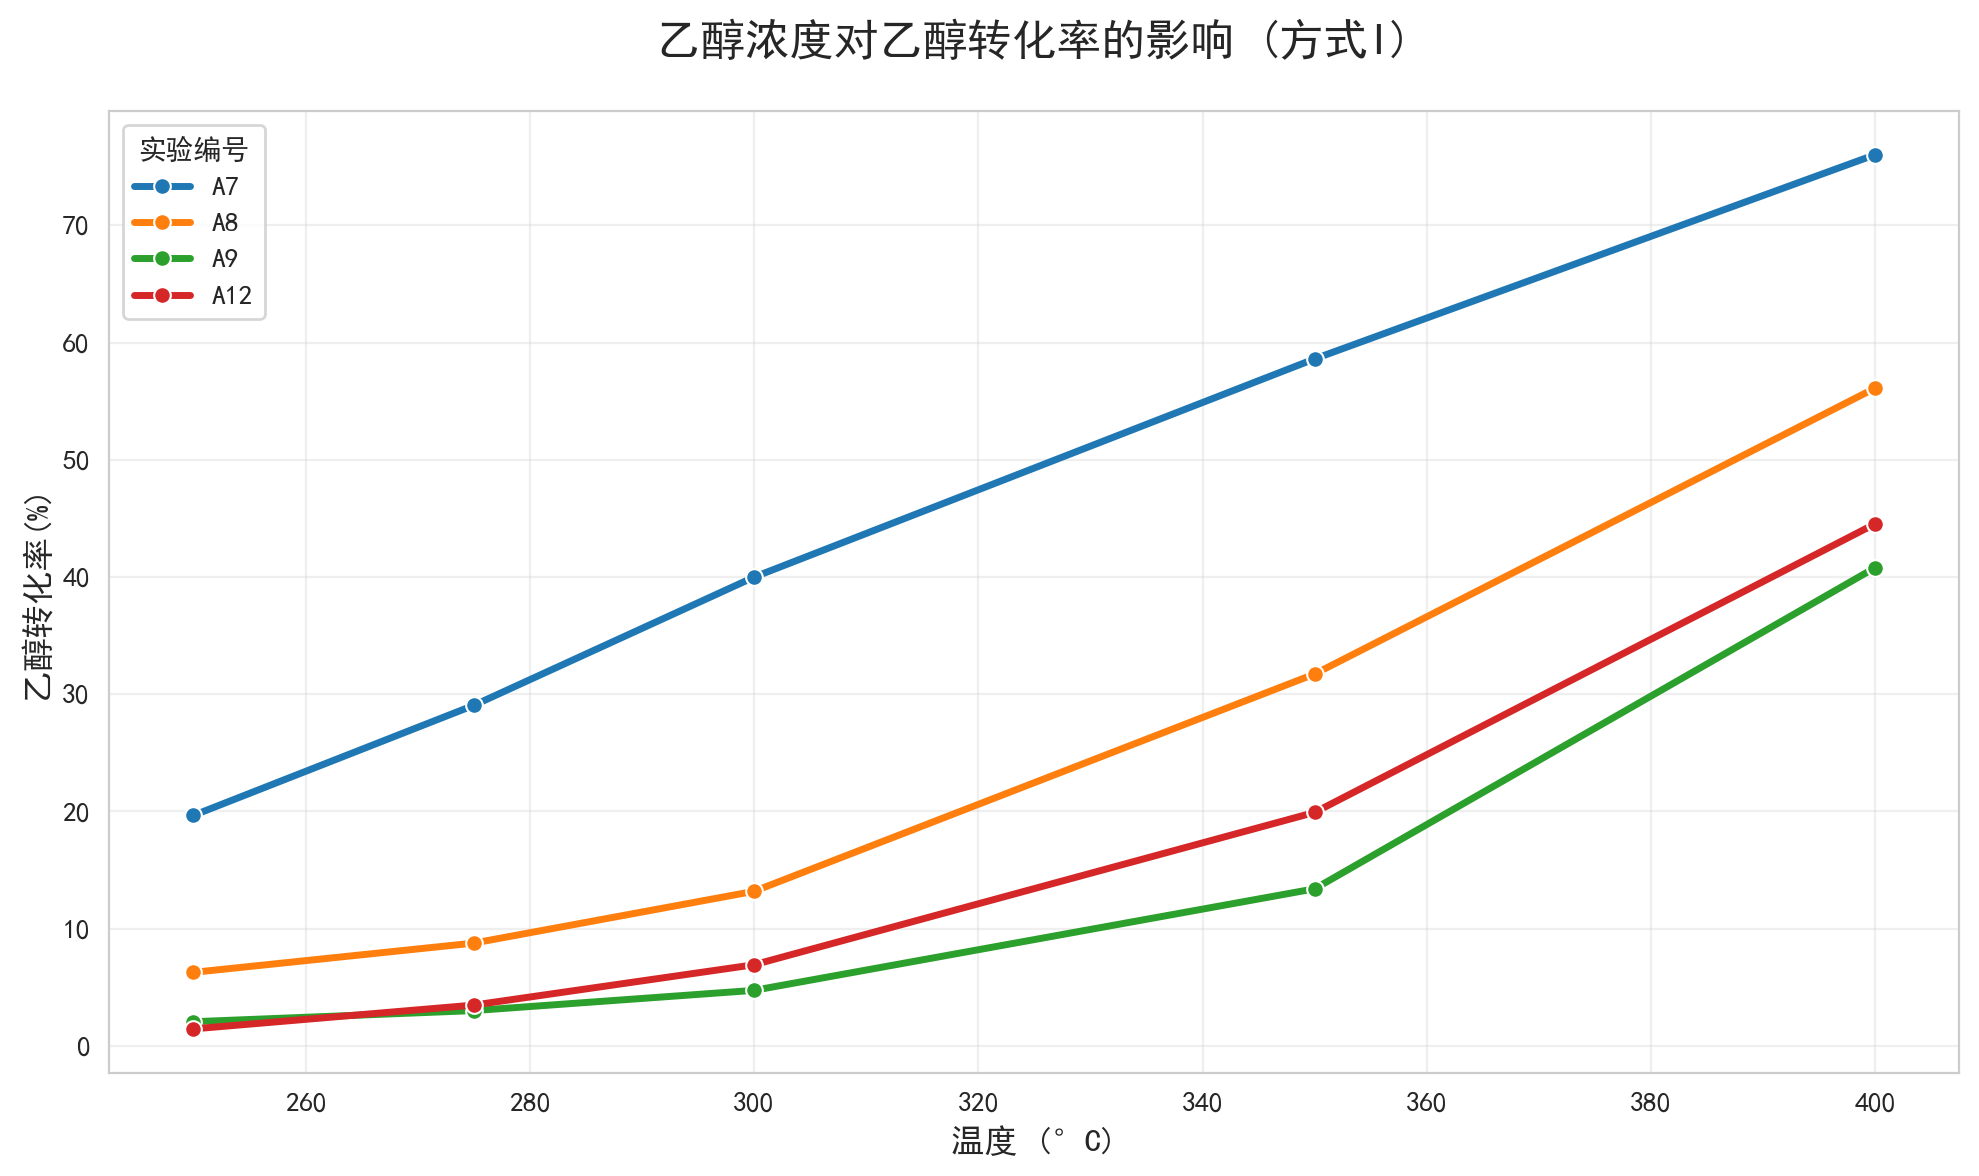
\includegraphics [scale=0.6]{图/2-2-3-2.png}
	\caption{乙醇浓度对乙醇转化率的影响 (方式I)} 
	\label{fig:1}
\end{figure}

\begin{figure}[h]%[h]:固定作用
	\centering%置中
	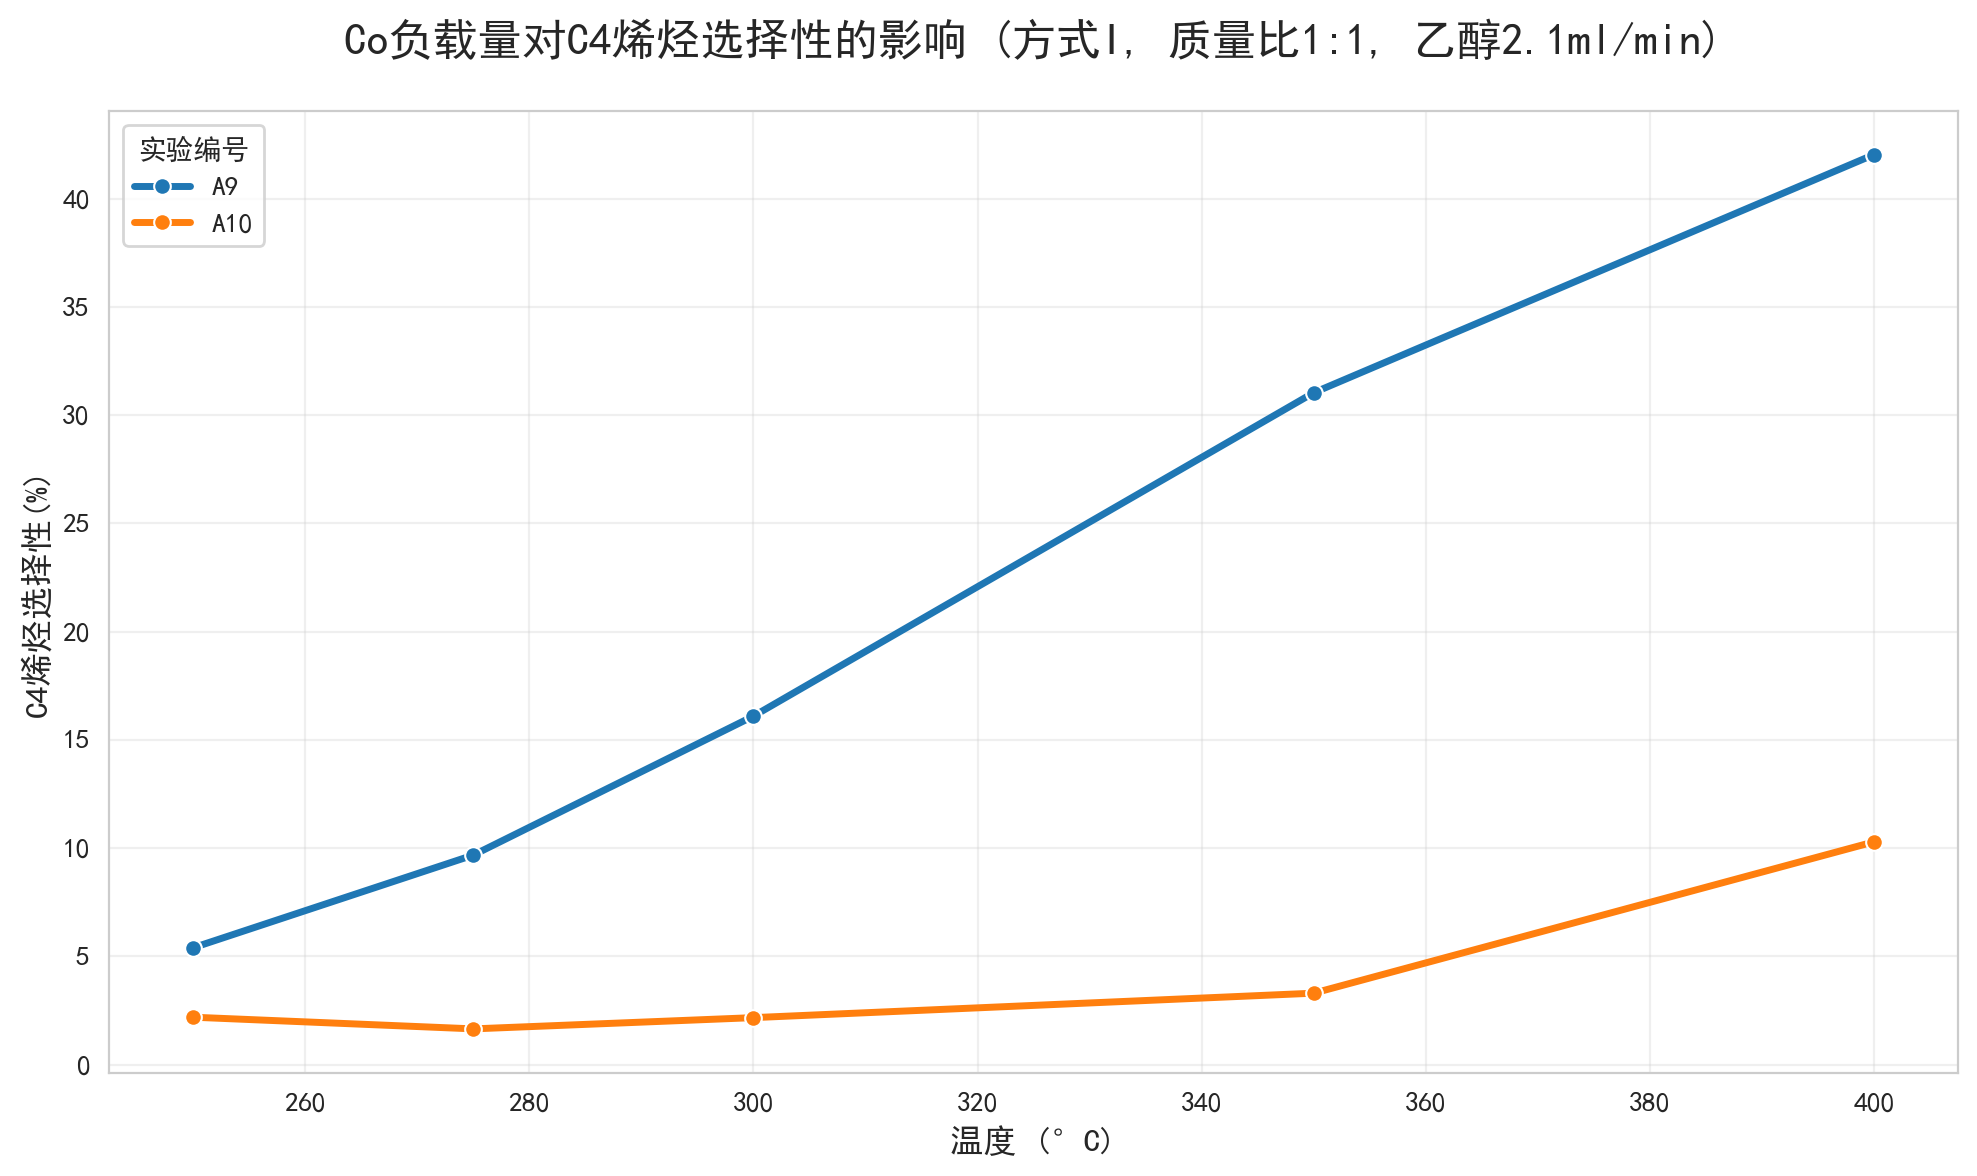
\includegraphics [scale=0.6]{图/2-3-2-1.png}
	\caption{乙醇浓度对C4烯烃选择性的影响 (方式I)} 
	\label{fig:1}
\end{figure}

\begin{figure}[h]%[h]:固定作用
	\centering%置中
	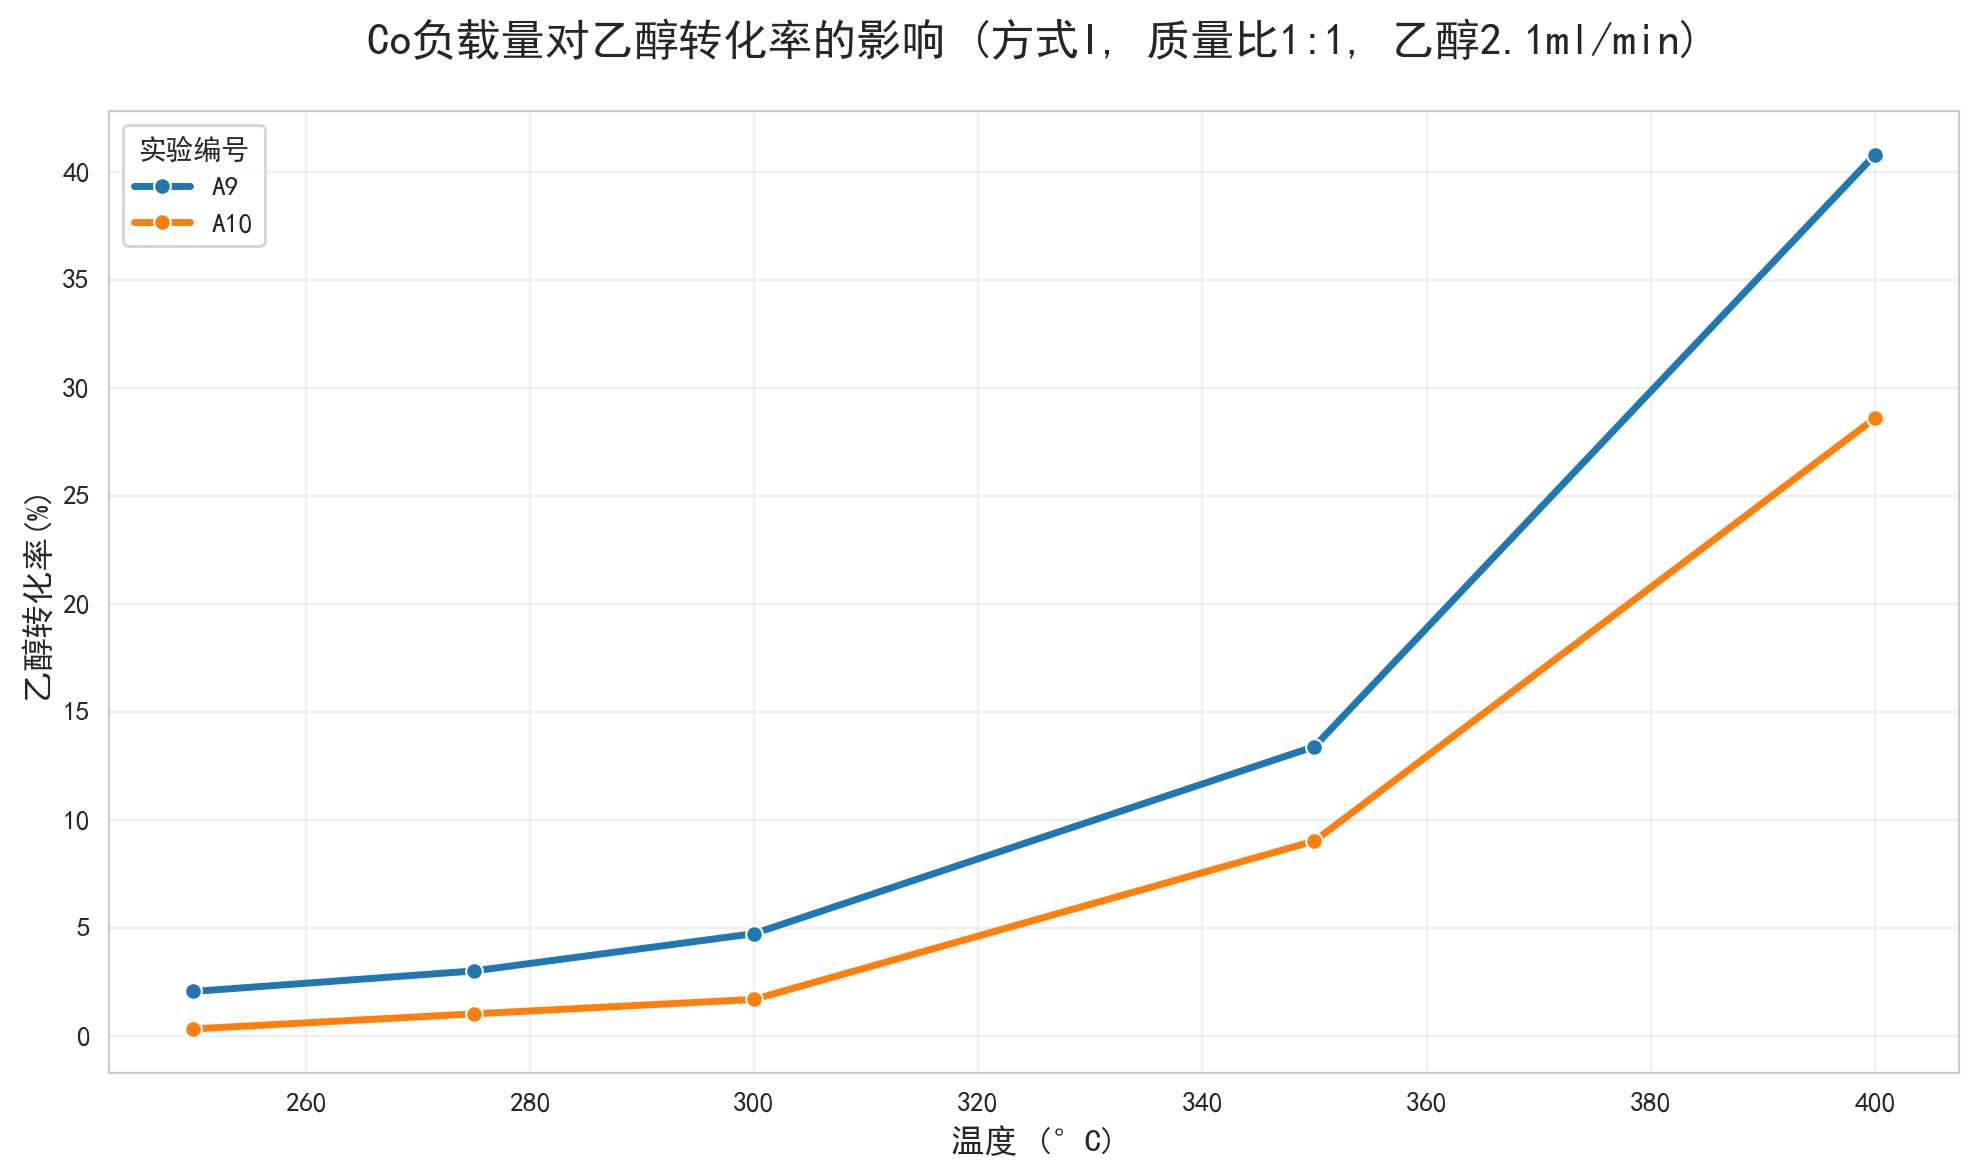
\includegraphics [scale=0.6]{图/2-3-2-2.png}
	\caption{乙醇浓度对乙醇转化率的影响 (方式I)} 
	\label{fig:1}
\end{figure}

\begin{figure}[h]%[h]:固定作用
	\centering%置中
	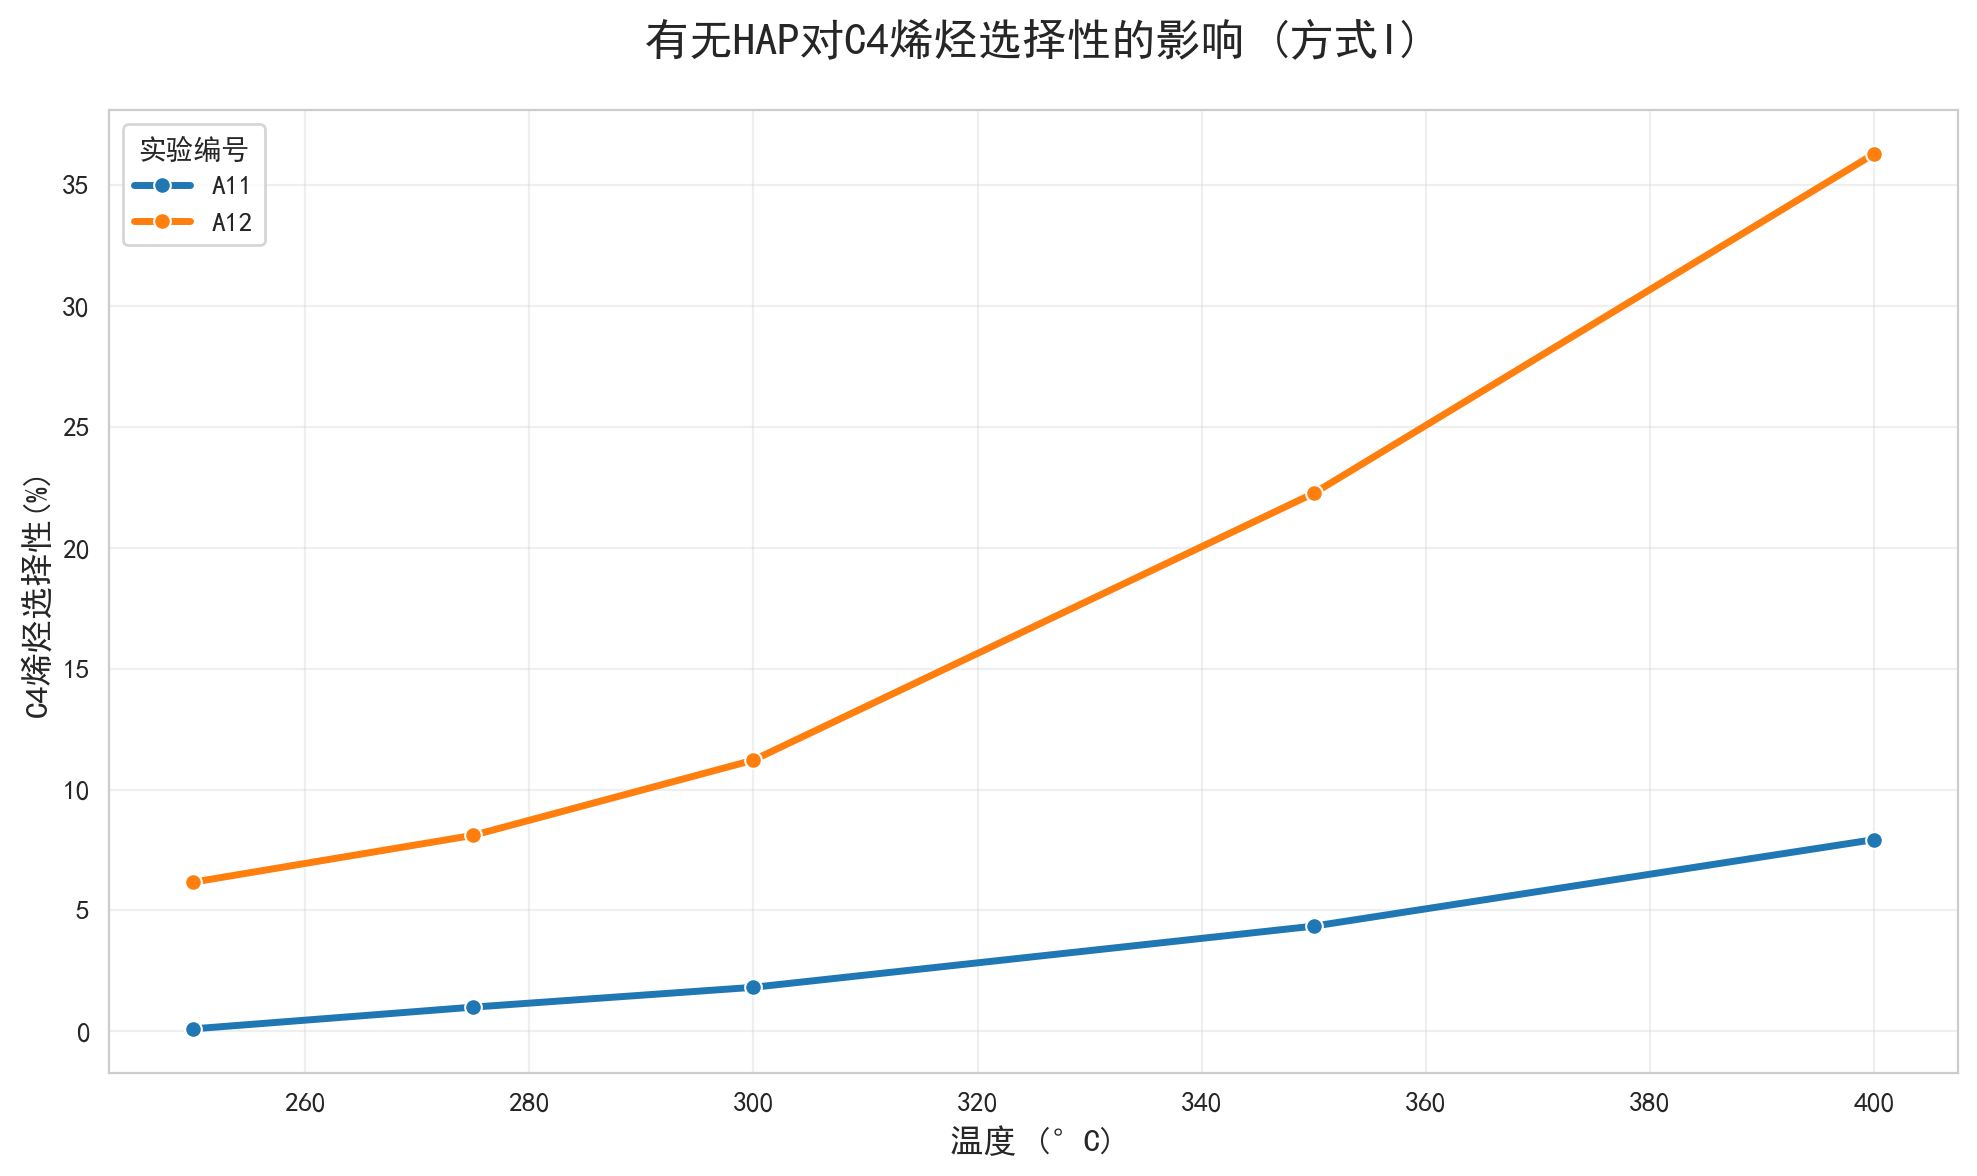
\includegraphics [scale=0.6]{图/2-4-1-1.png}
	\caption{有无HAP对C4烯烃选择性的影响 (方式I)} 
	\label{fig:1}
\end{figure}

\begin{figure}[h]%[h]:固定作用
	\centering%置中
	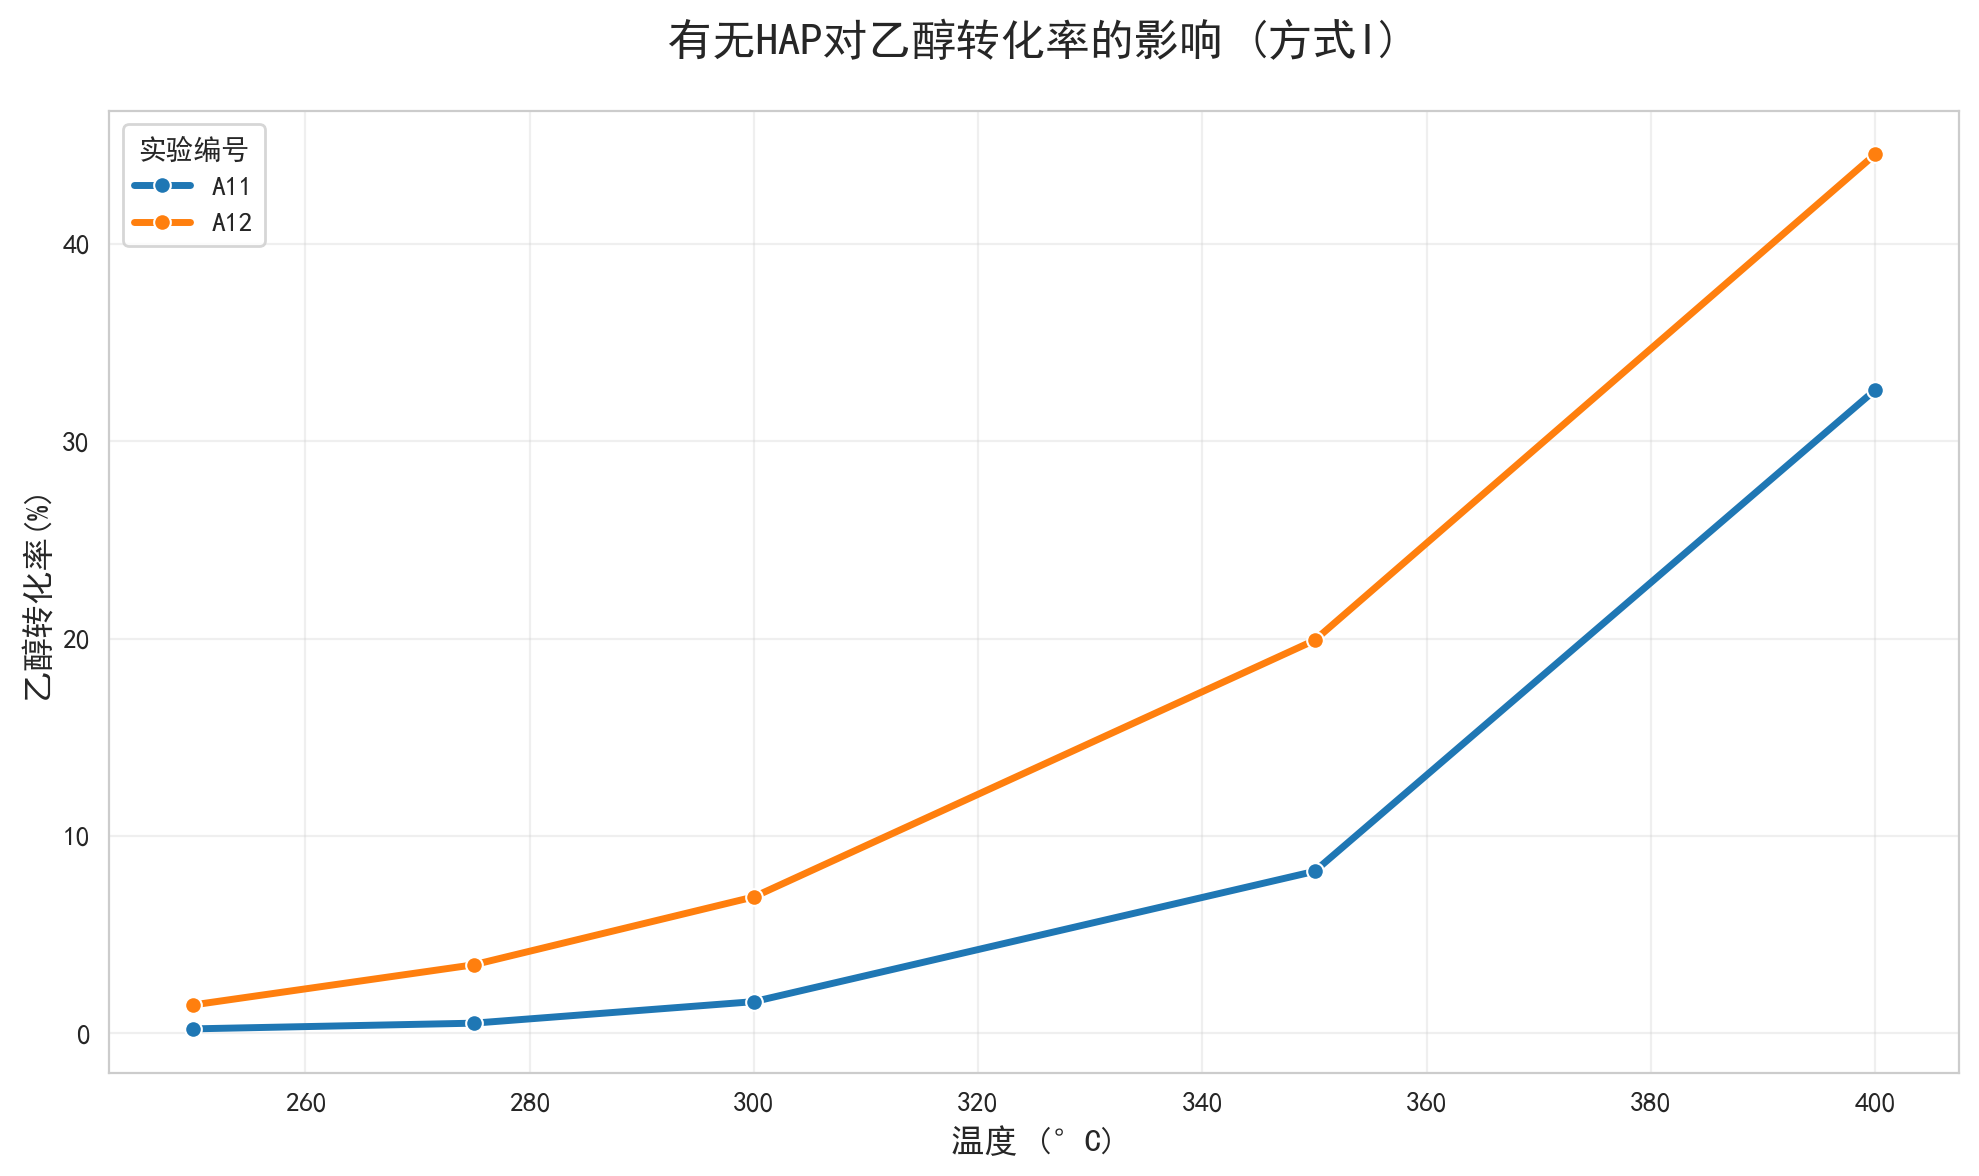
\includegraphics [scale=0.6]{图/2-4-1-2.png}
	\caption{有无HAP对乙醇转化率的影响 (方式I)} 
	\label{fig:1}
\end{figure}

\begin{figure}[h]%[h]:固定作用
	\centering%置中
	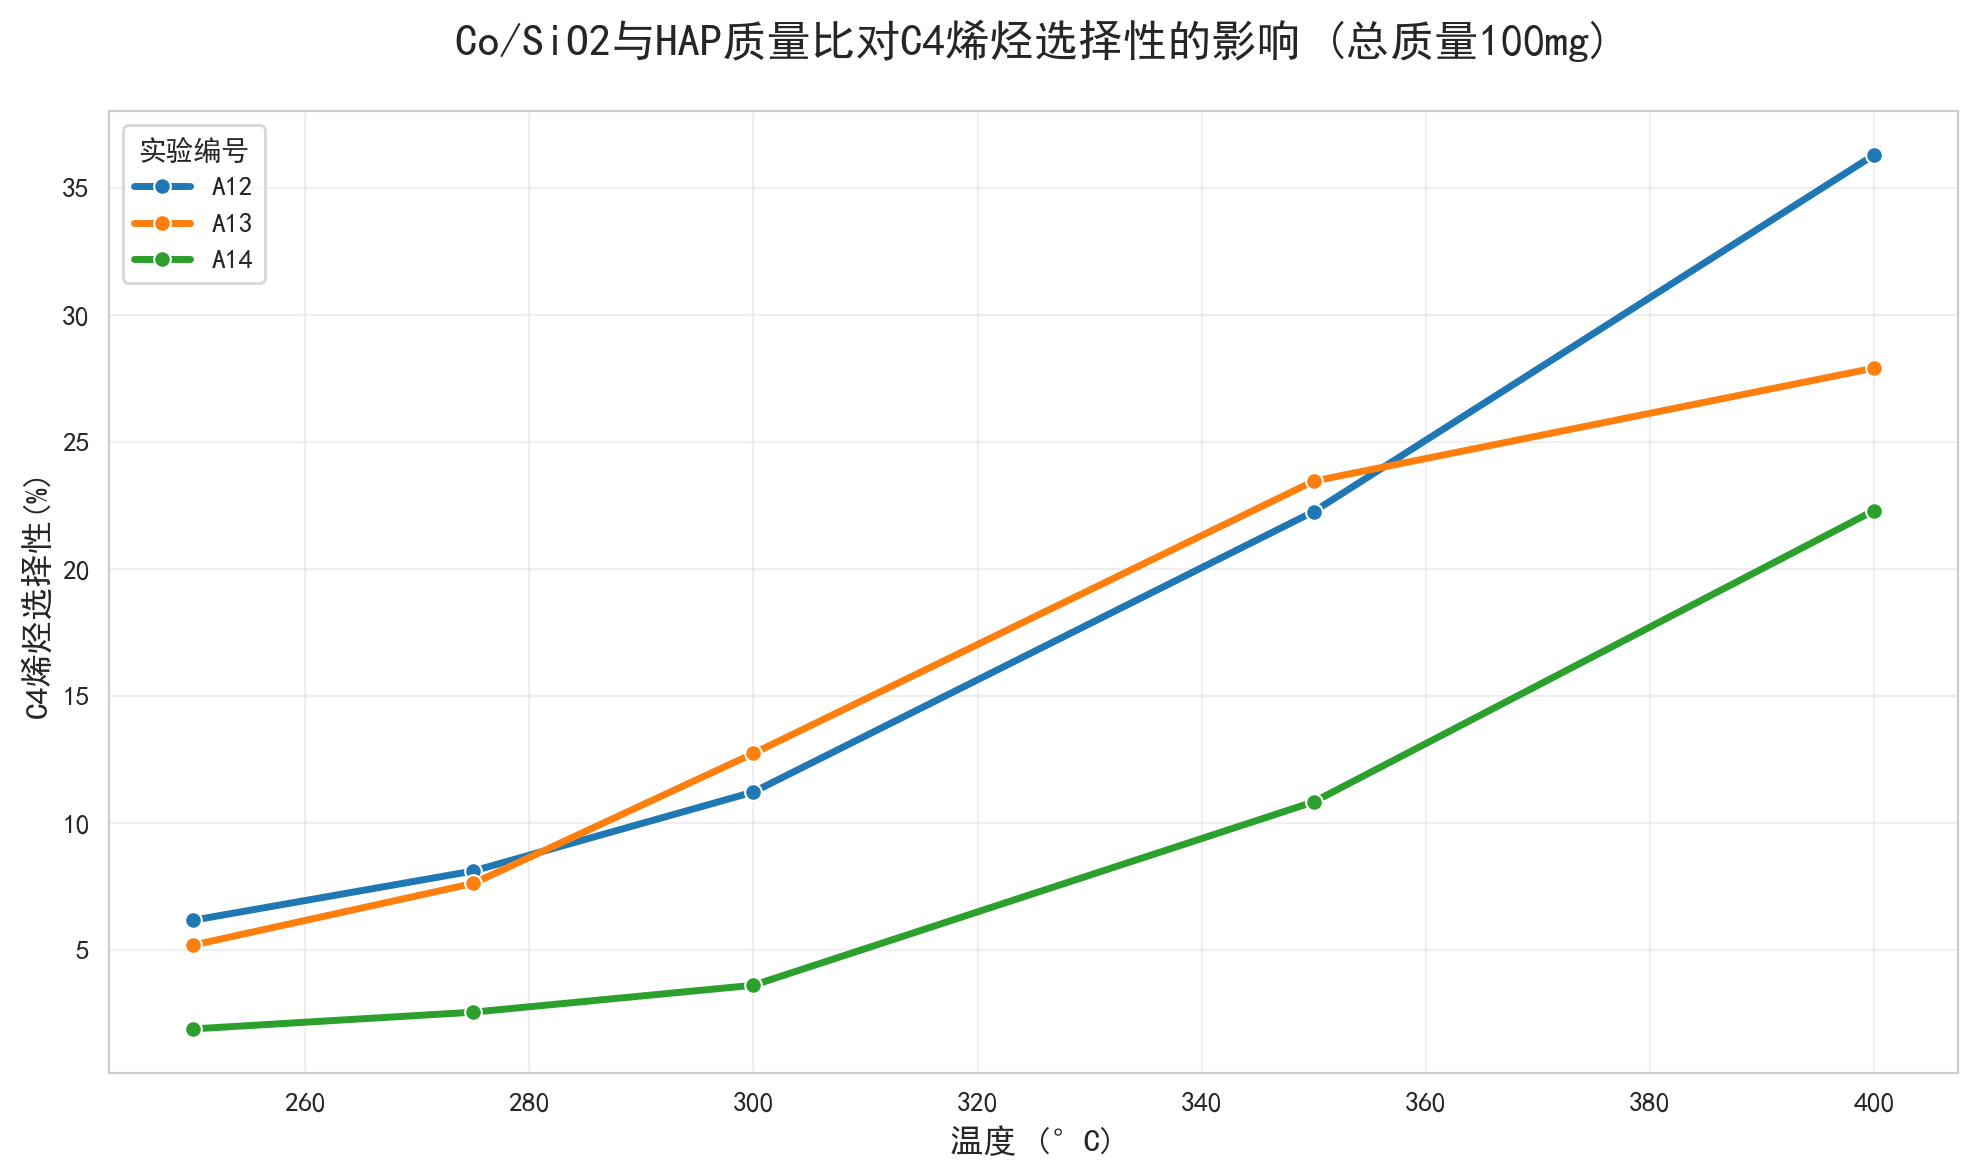
\includegraphics [scale=0.6]{图/2-5-1-1.png}
	\caption{Co/SiO2与HAP质量比对C4烯烃选择性的影响 (总质量100mg)} 
	\label{fig:1}
\end{figure}

\begin{figure}[h]%[h]:固定作用
	\centering%置中
	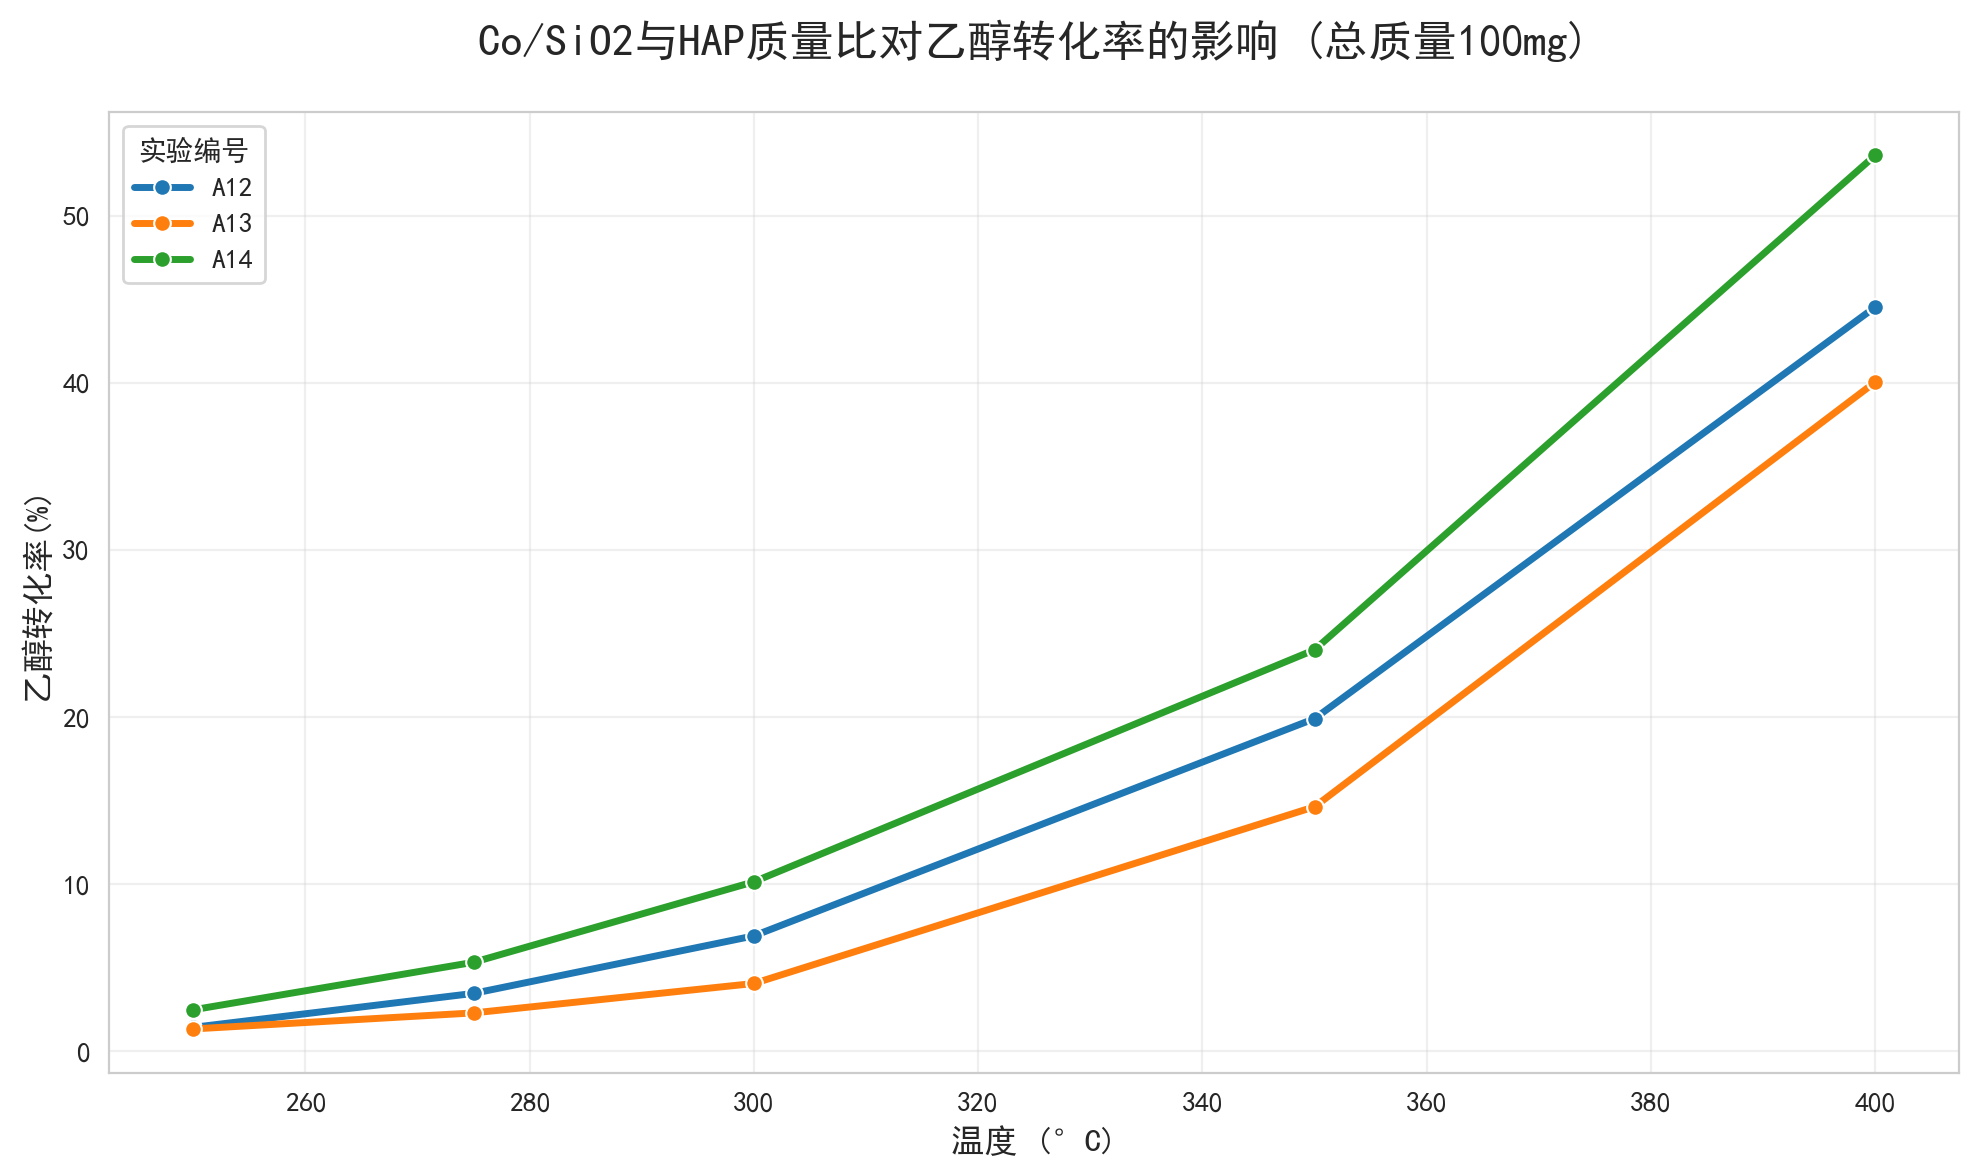
\includegraphics [scale=0.6]{图/2-5-1-2.png}
	\caption{Co/SiO2与HAP质量比对乙醇转化率的影响 (总质量100mg)} 
	\label{fig:1}
\end{figure}

\begin{figure}[h]%[h]:固定作用
	\centering%置中
	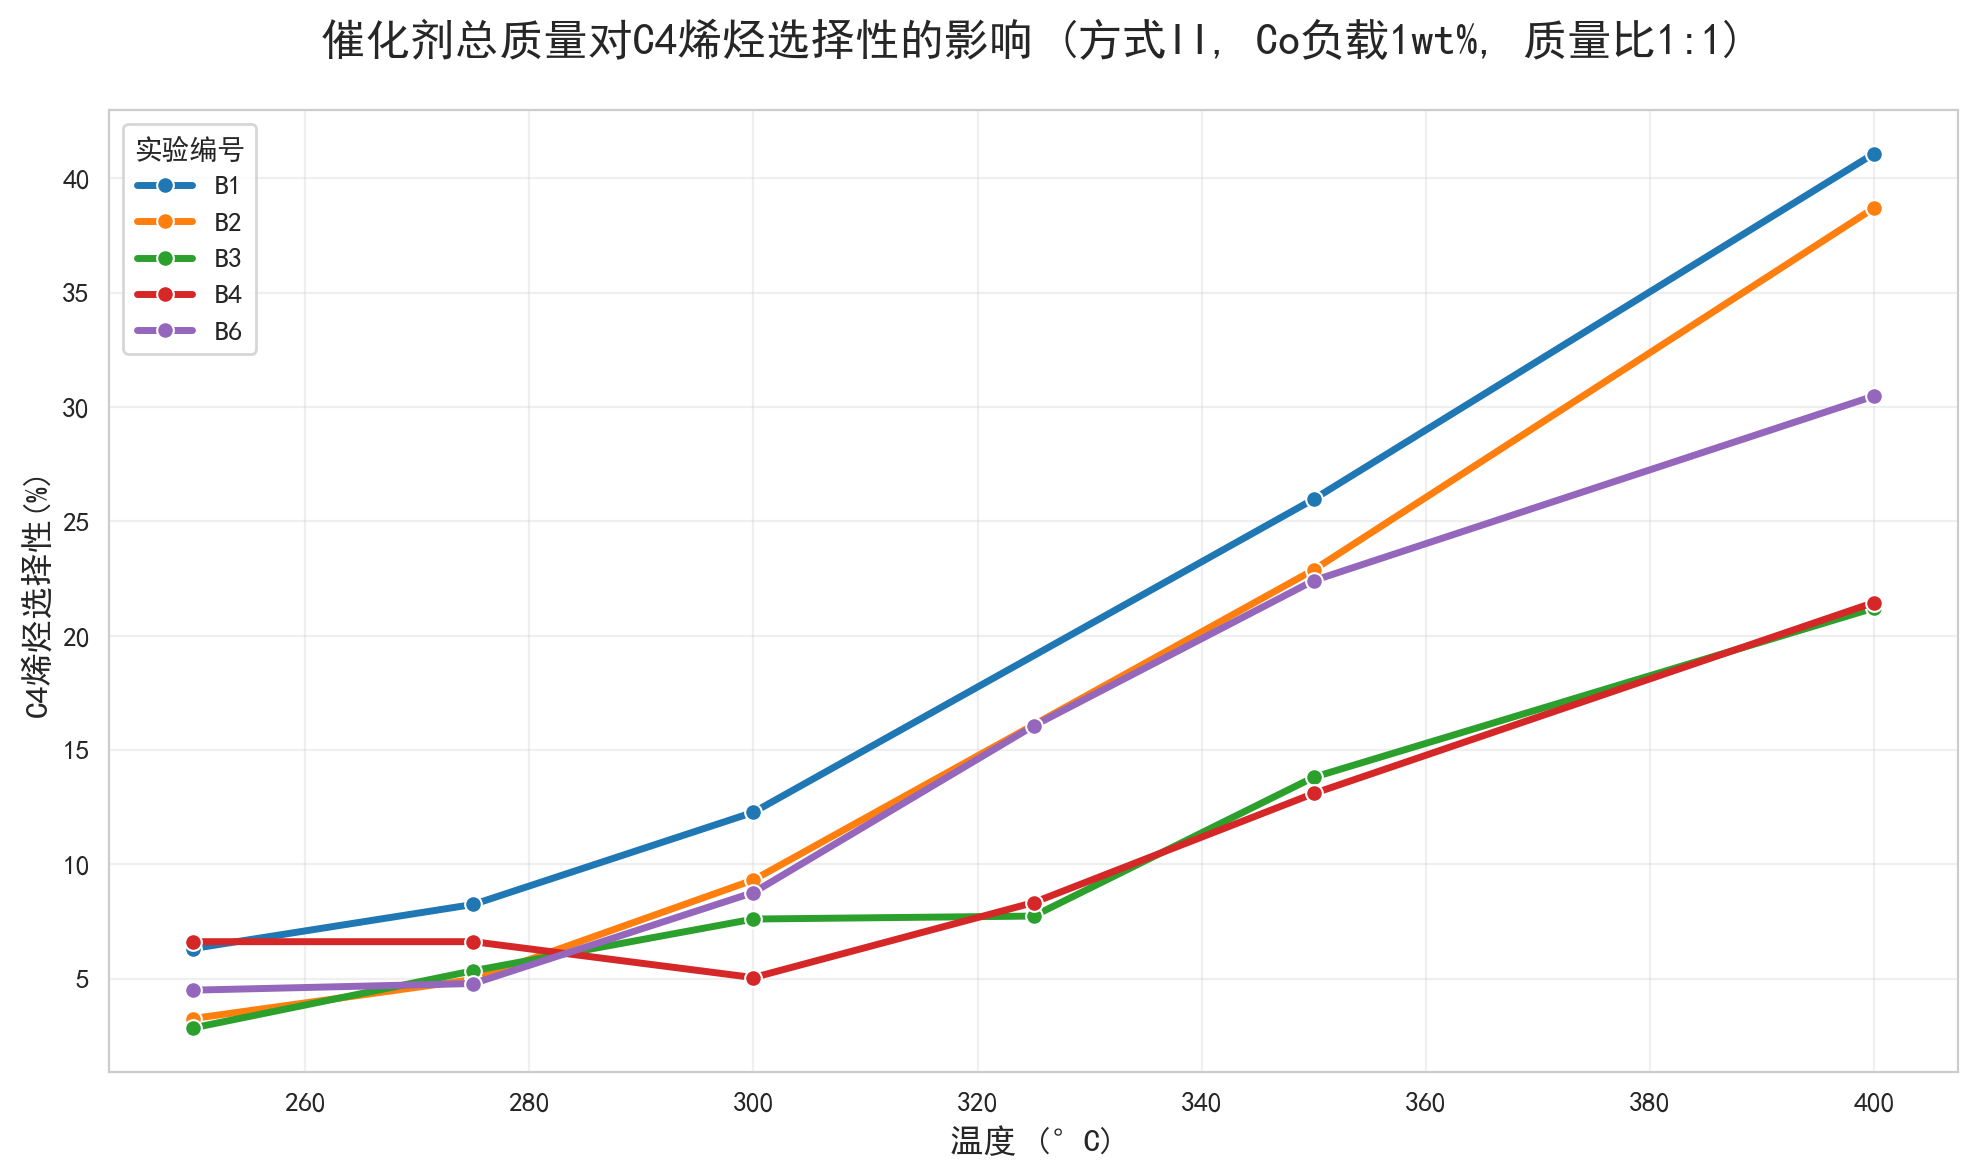
\includegraphics [scale=0.6]{图/2-6-1-1.png}
	\caption{催化剂总质量对C4烯烃选择性的影响 (方式II, Co负载1wt\%, 质量比1:1)} 
	\label{fig:1}
\end{figure}

\begin{figure}[h]%[h]:固定作用
	\centering%置中
	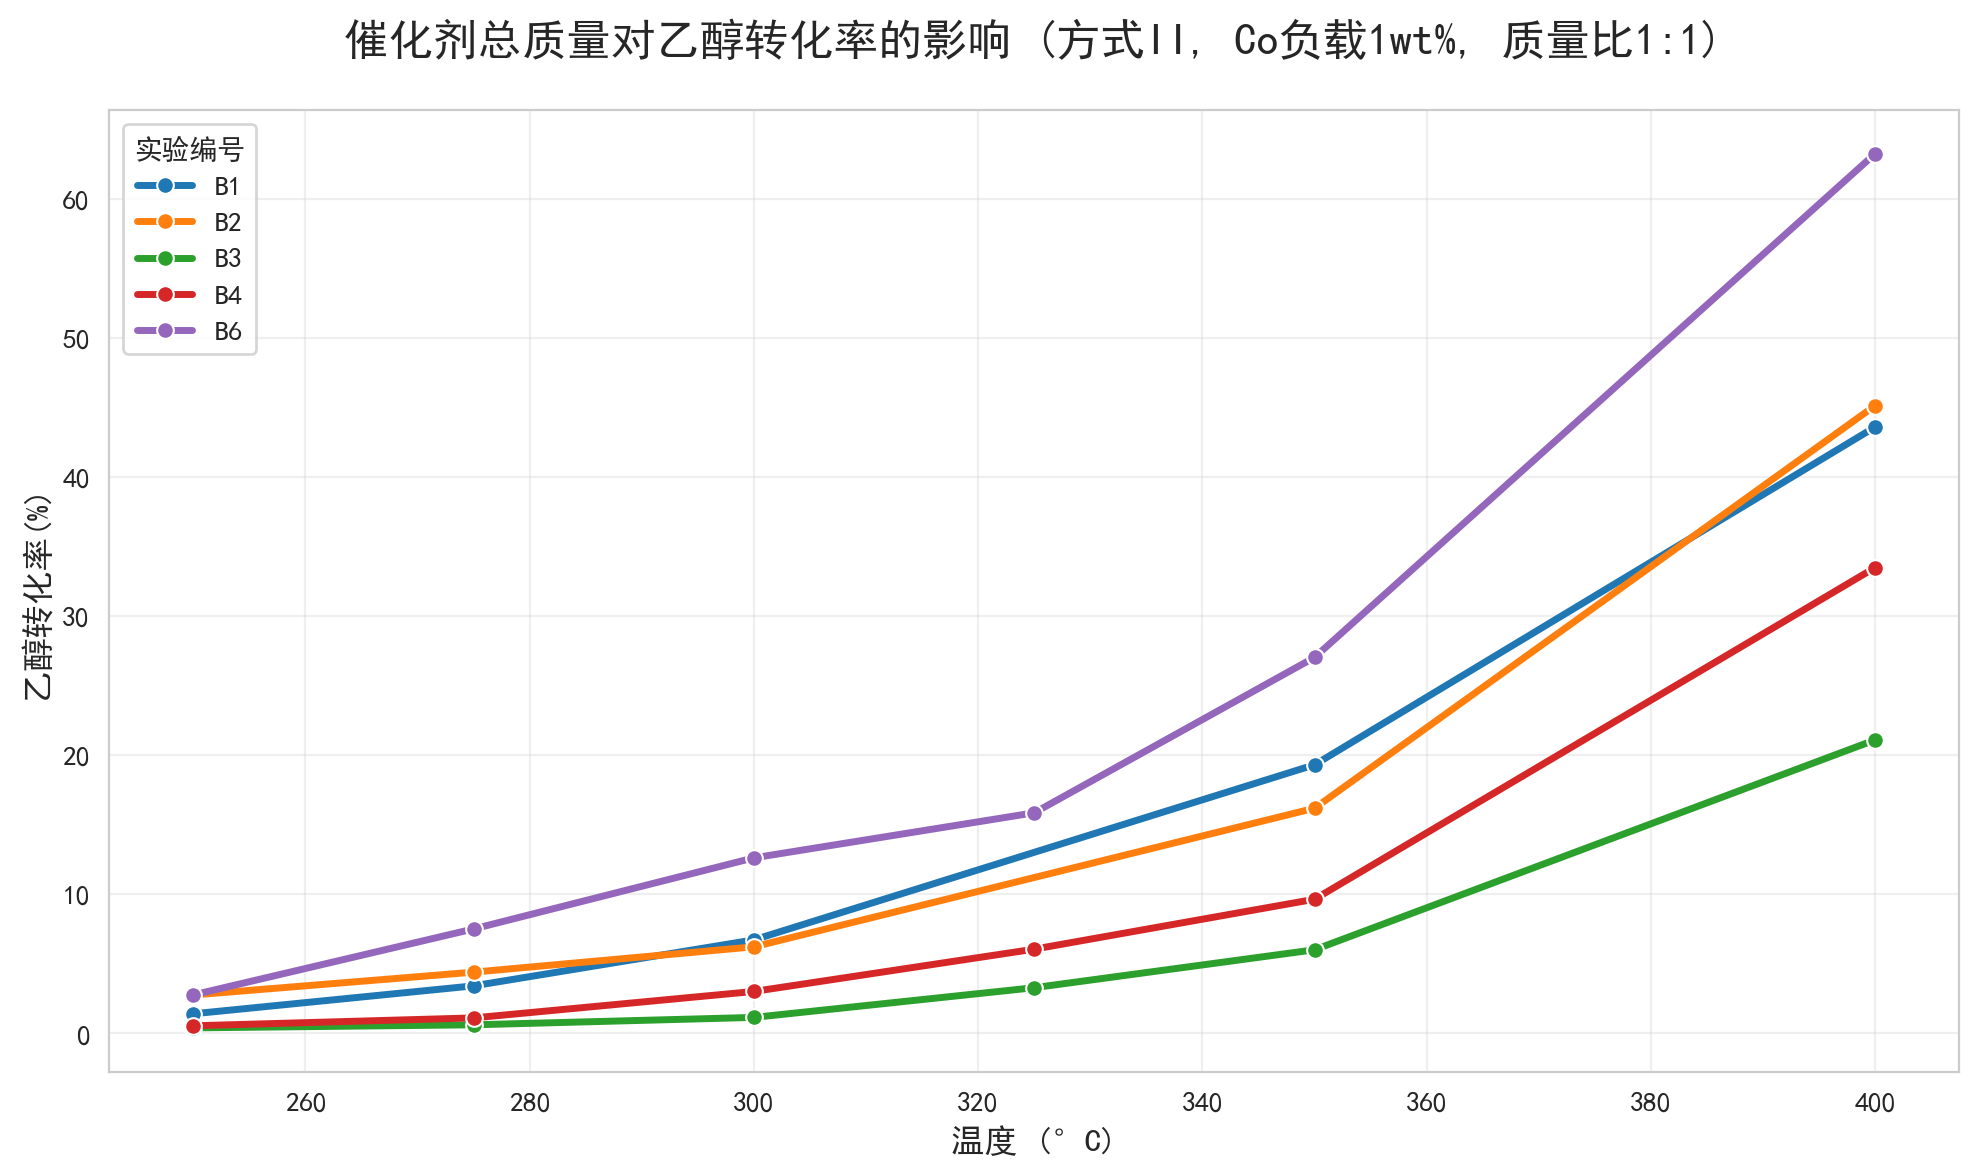
\includegraphics [scale=0.6]{图/2-6-1-2.png}
	\caption{催化剂总质量对乙醇转化率的影响 (方式II, Co负载1wt\%, 质量比1:1)} 
	\label{fig:1}
\end{figure}

\begin{figure}[h]%[h]:固定作用
	\centering%置中
	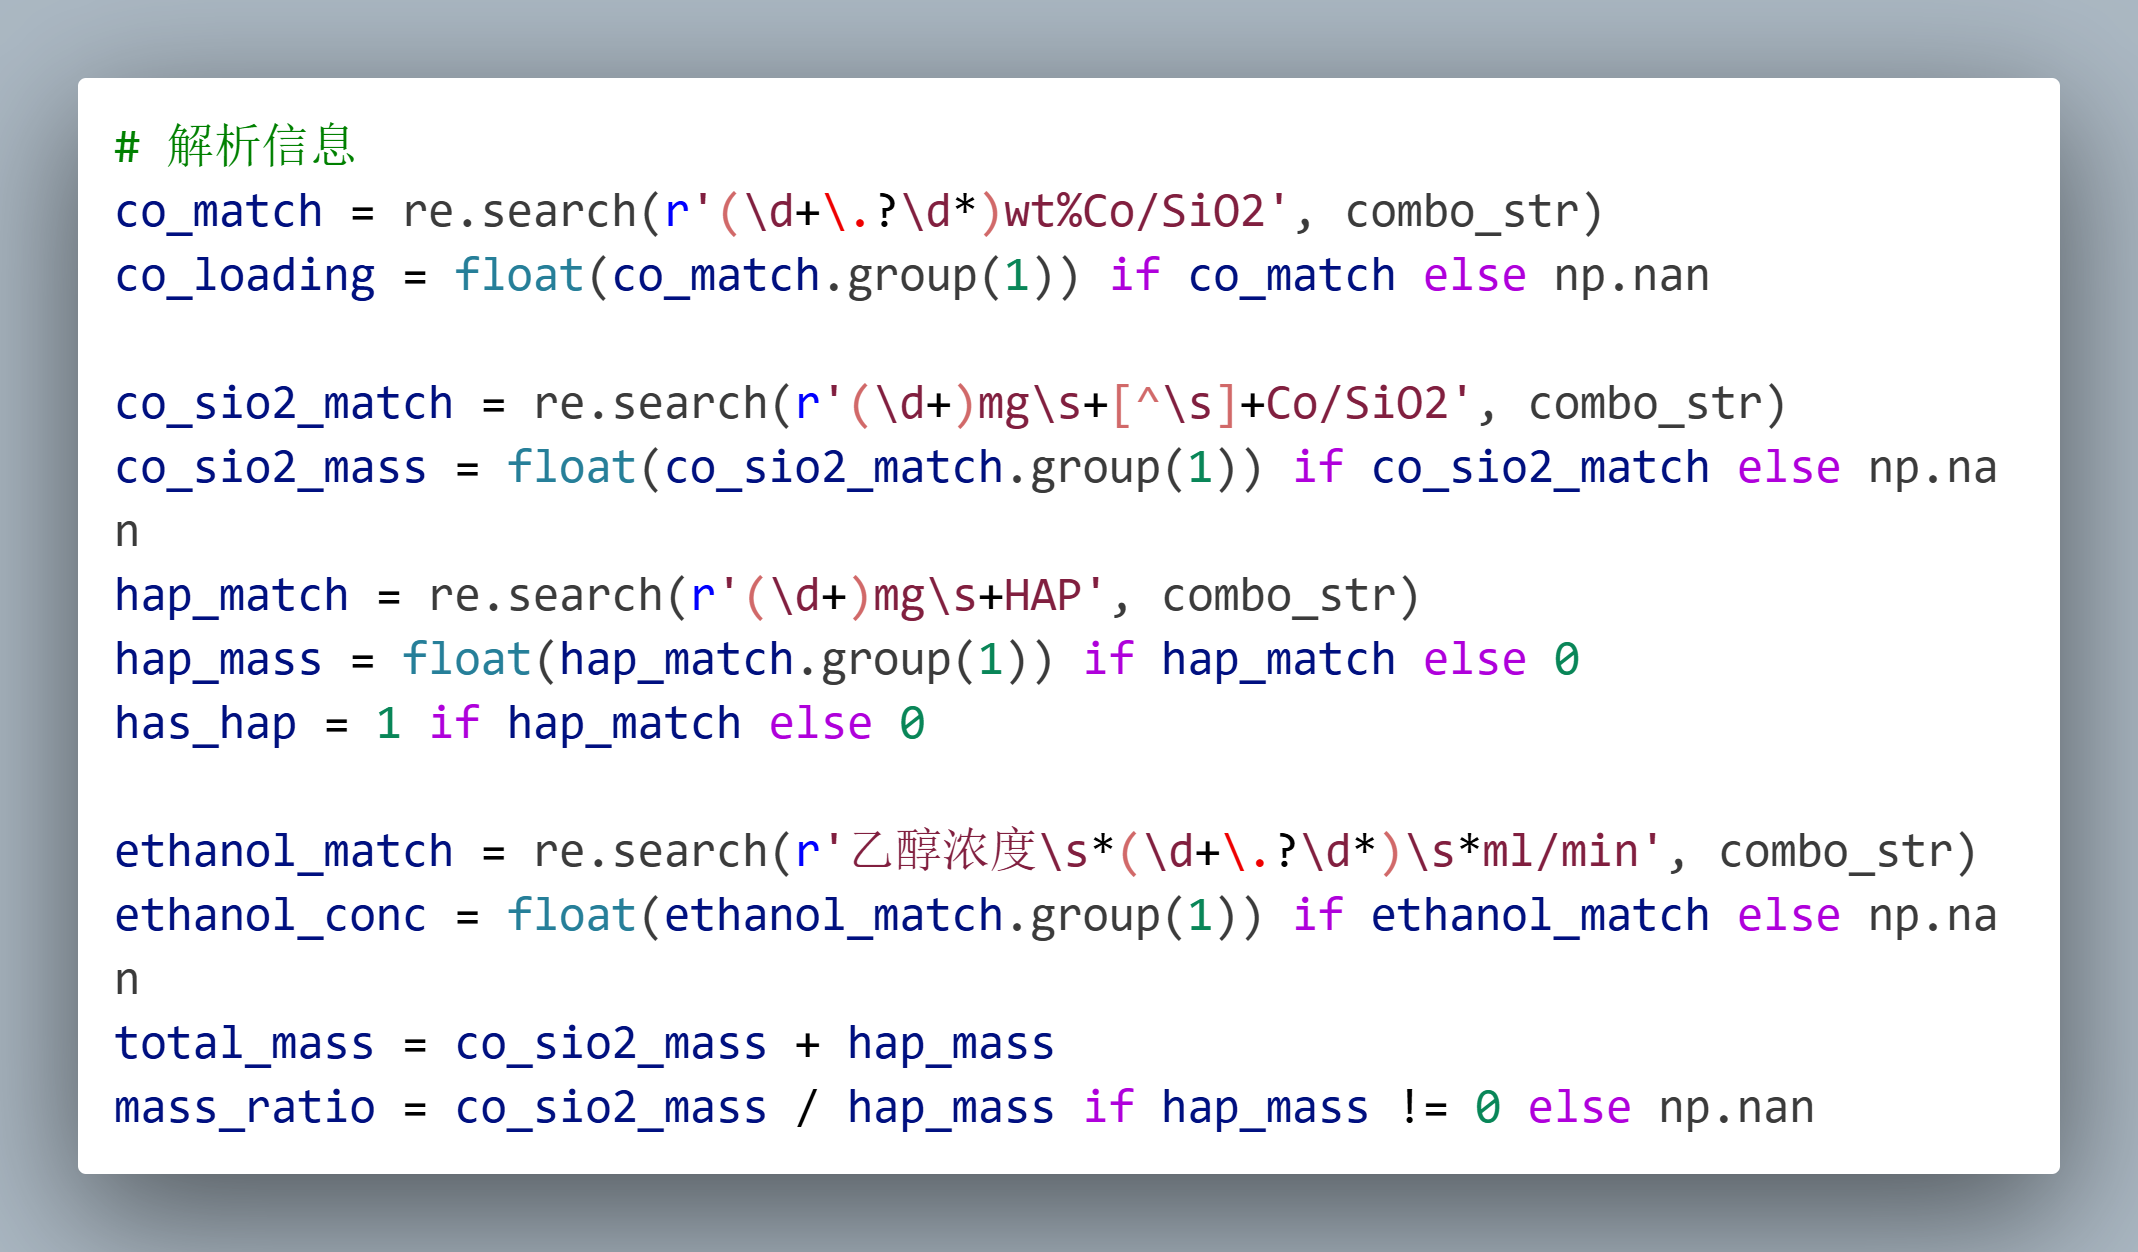
\includegraphics [scale=0.2]{图/code_1.png}
	\caption{Python正则化表达式代码} 
	\label{fig:1}
\end{figure}

\begin{figure}[h]%[h]:固定作用
	\centering%置中
	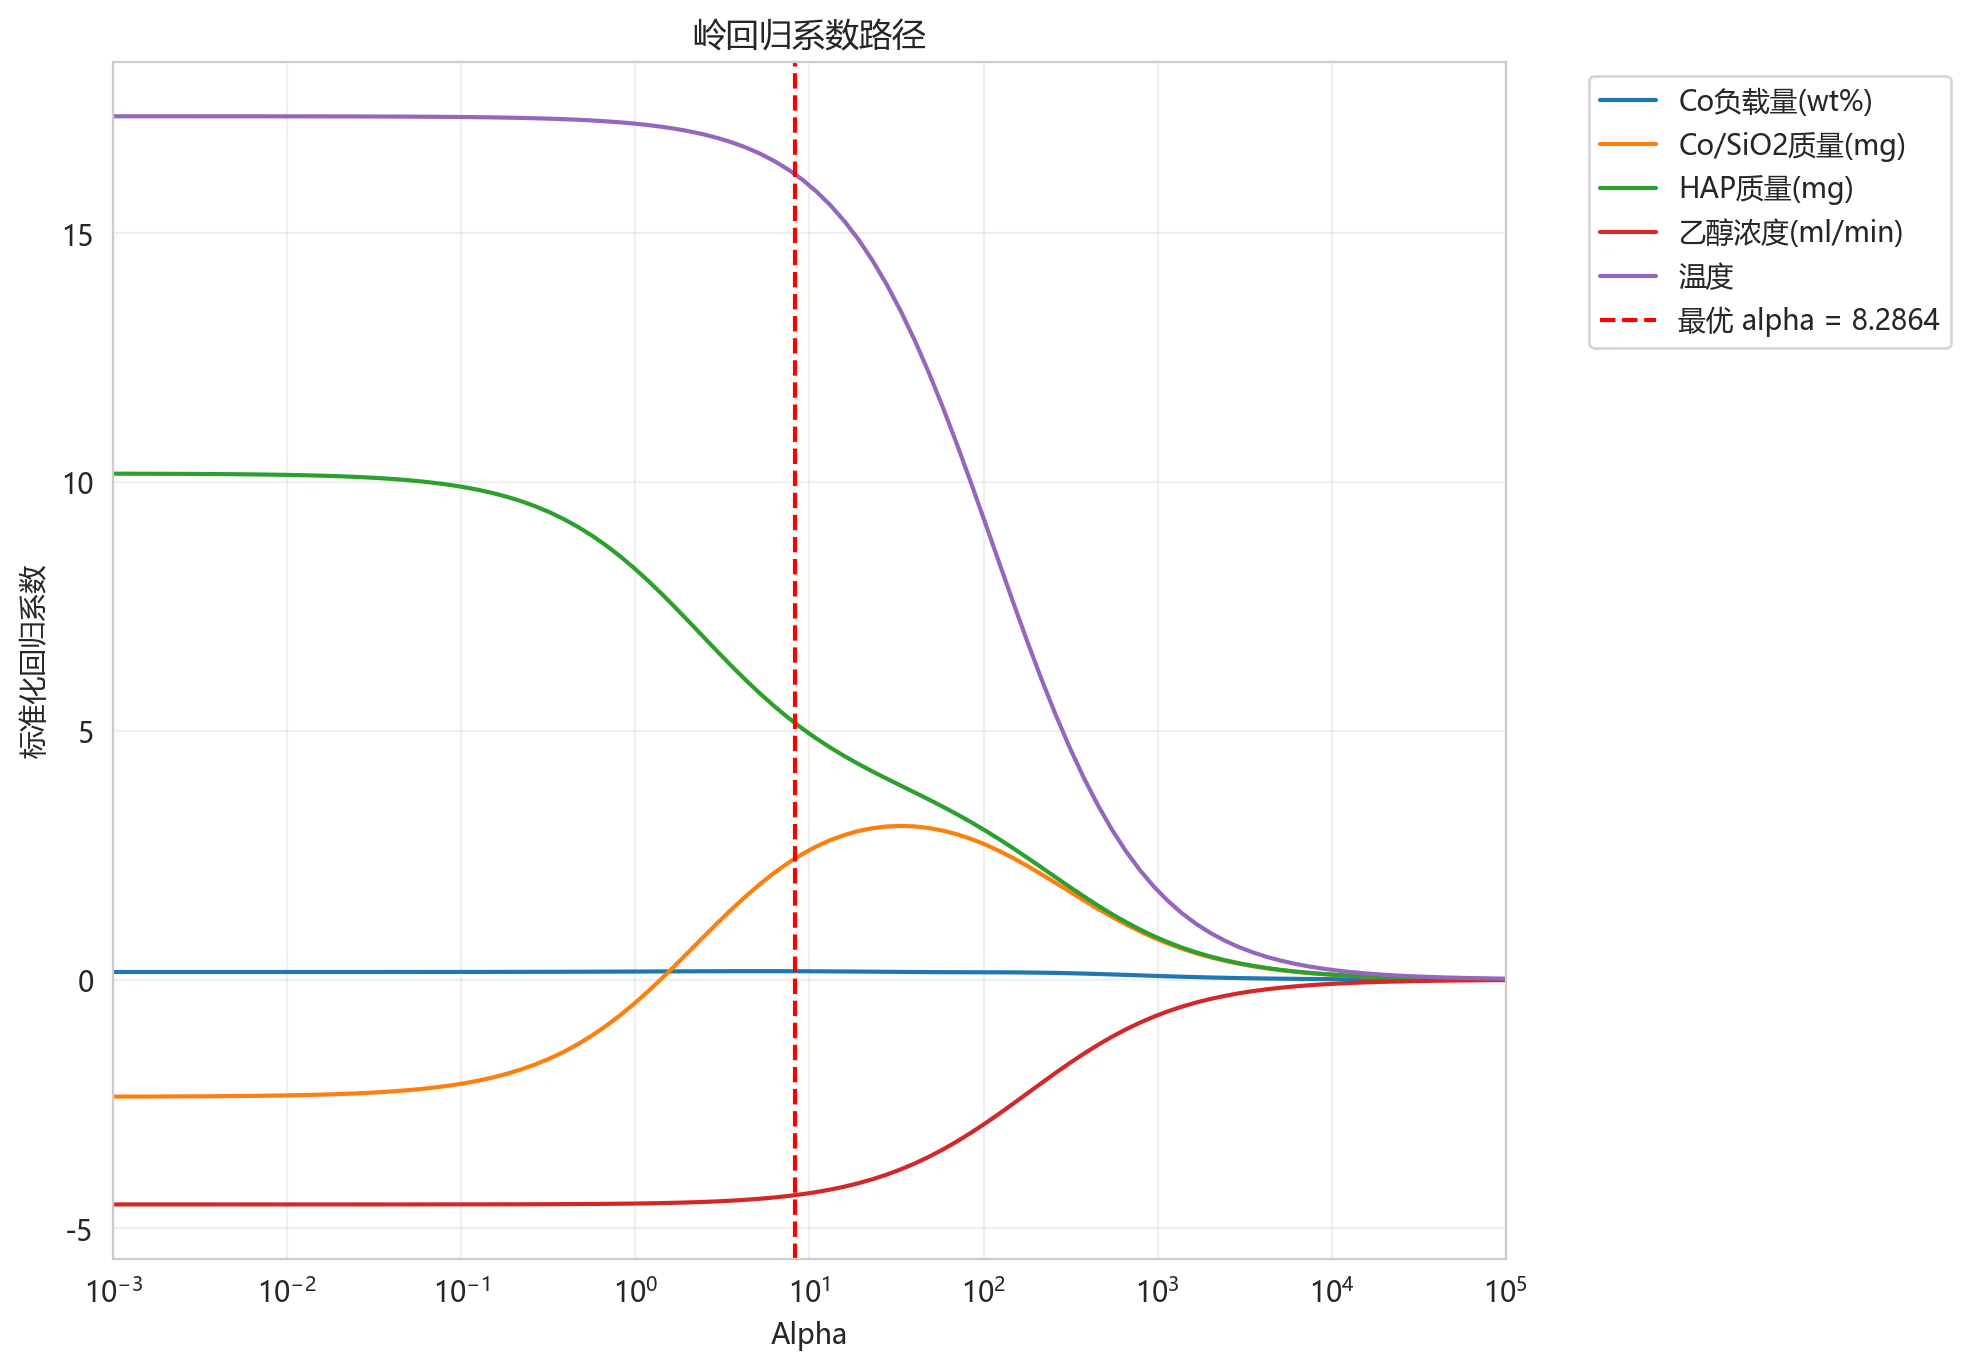
\includegraphics [scale=0.6]{图/ling-yichun.png}
	\caption{乙醇转化率岭回归系数路径} 
	\label{fig:1}
\end{figure}

\begin{table}[!htbp]
	\caption{乙醇转化率模型的标准化回归系数}
	\centering
	\begin{tabular}{l c}
		\hline
		\multicolumn{1}{c}{\textbf{特征名称}} & \textbf{标准化回归系数} \\
		\hline
		Co负载量(wt\%)      & 0.1697 \\
		Co/SiO2质量(mg)     & 2.4395 \\
		HAP质量(mg)         & 5.1538 \\
		乙醇浓度(ml/min)    & -4.3307 \\
		温度 (°C)                & 16.1869 \\
		\hline
		\label{tab:ridge_coefficients}
	\end{tabular}
\end{table}

\begin{figure}[h]%[h]:固定作用
	\centering%置中
	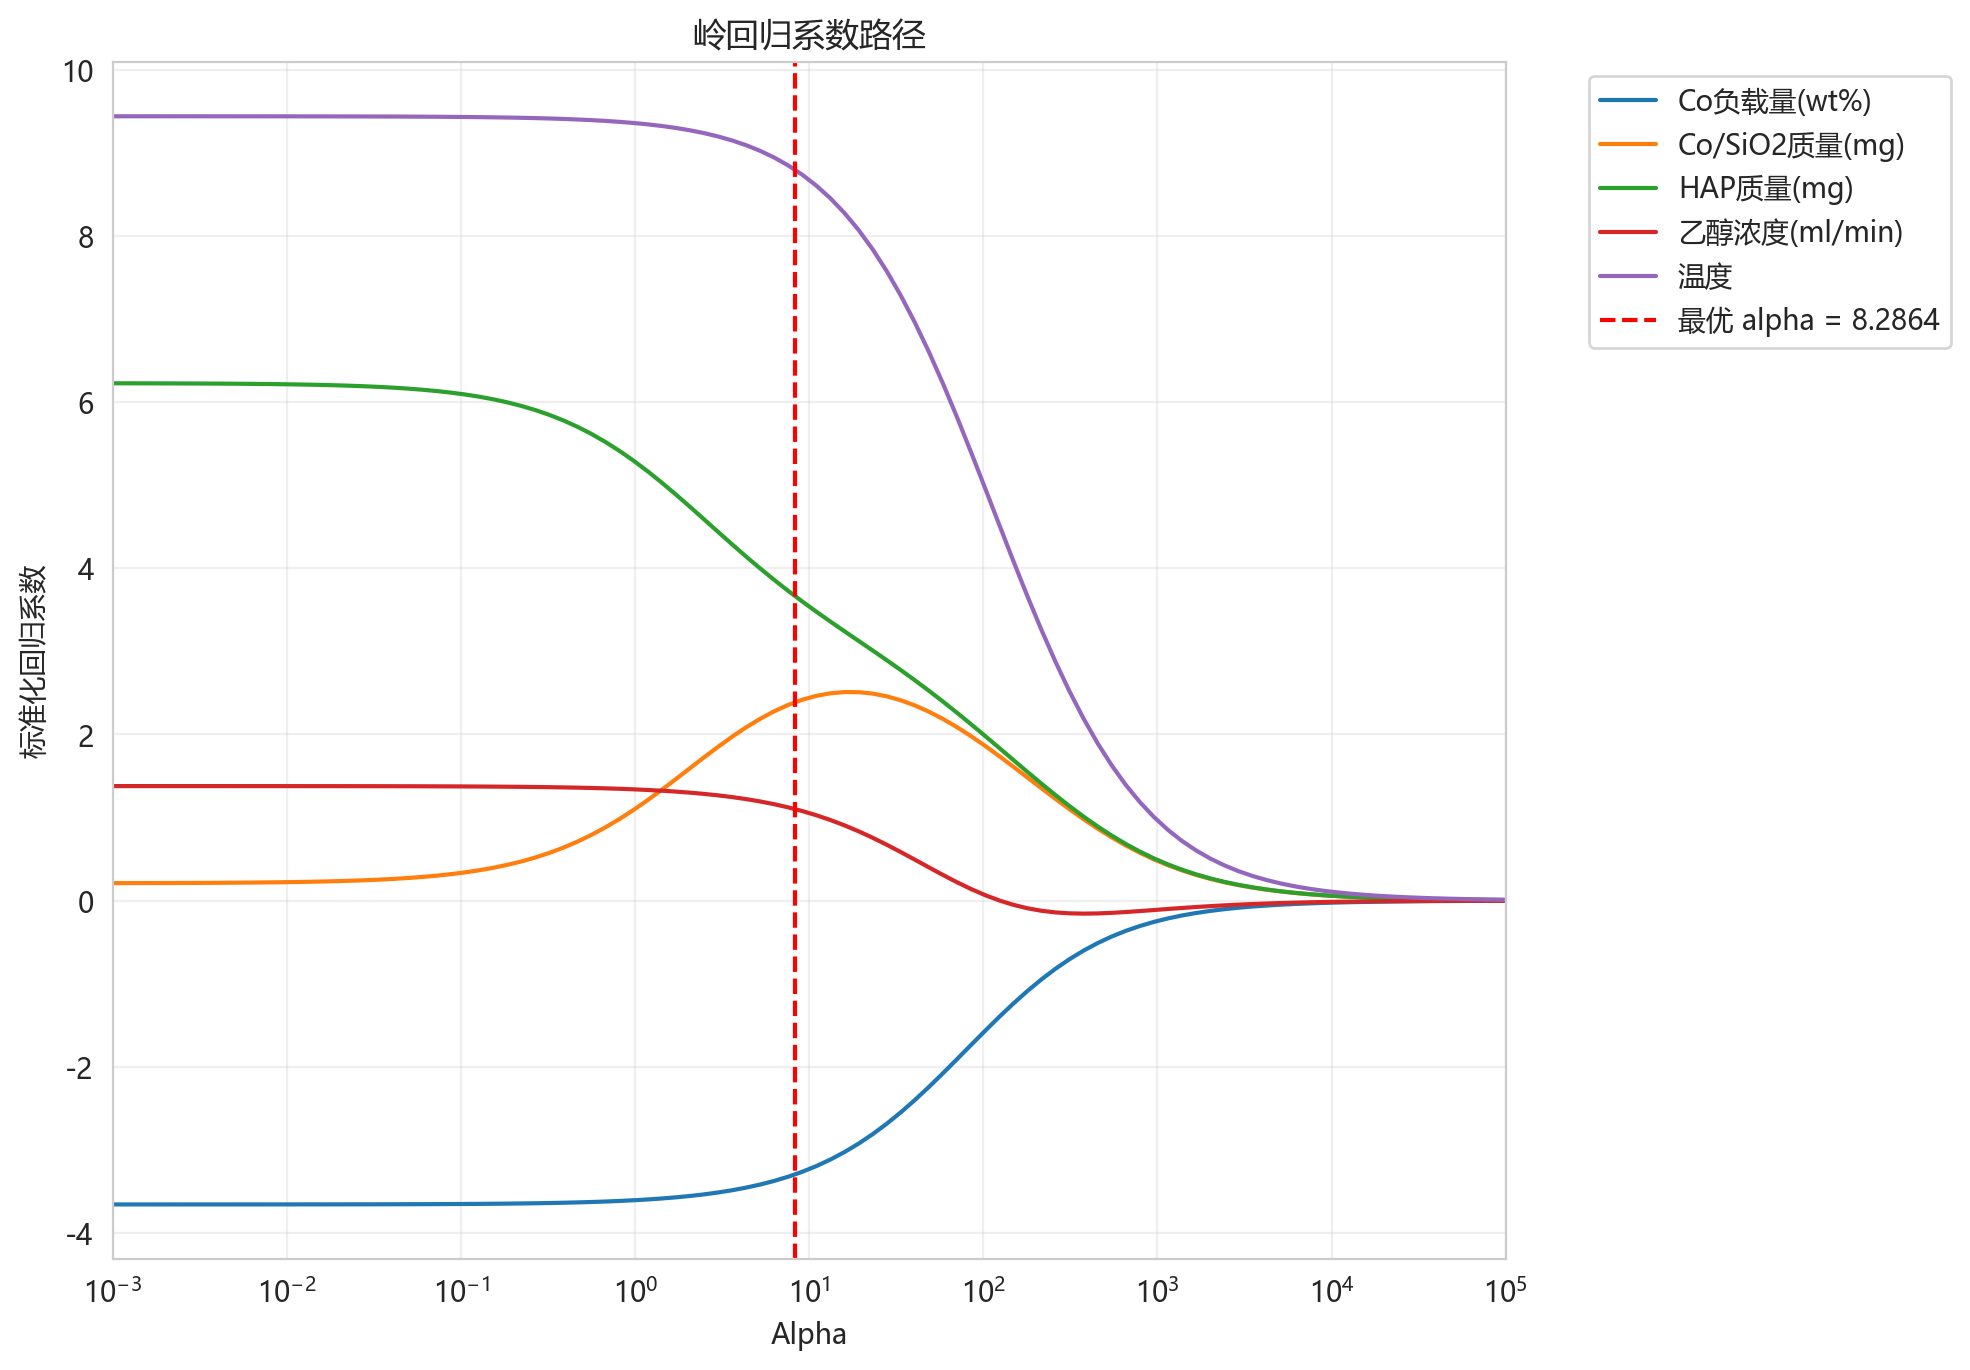
\includegraphics [scale=0.6]{图/ling-xuanzexing.png}
	\caption{ \( \text{C}_4 \) 烯烃选择性岭回归系数路径} 
	\label{fig:1}
\end{figure}

\begin{table}[!htbp]
	\caption{C4烯烃选择性模型的标准化回归系数}
	\centering
	\begin{tabular}{l c}
		\hline
		\multicolumn{1}{c}{\textbf{特征名称}} & \textbf{标准化回归系数} \\
		\hline
		Co负载量(wt\%)      & -3.4383 \\
		Co/SiO2质量(mg)     & 2.1327 \\
		HAP质量(mg)         & 4.0744 \\
		乙醇浓度(ml/min)    & 1.2088 \\
		温度 (°C)               & 9.0609 \\
		\hline
		\label{tab:ridge_selectivity}
	\end{tabular}
\end{table}



